%%-----------------------------------------------------------------------%%
%%--- Introduction to Graph Theory --------------------------------------%%

\chapter{Introduction to Graph Theory}
\label{chap:introduction}

Our journey into graph theory starts with a puzzle that was solved
over 250 years ago by
Leonhard Euler~(1707--1783)\index{Euler, Leonhard}. The Pregel River
flowed through the town of K\"onigsberg, which is present day
Kaliningrad in Russia. Two islands protruded from the river. On either
side of the mainland, two bridges joined one side of the mainland with
one island and a third bridge joined the same side of the mainland
with the other island. A bridge connected the two islands. In total,
seven bridges connected the two islands with both sides of the
mainland. A popular exercise among the citizens of K\"onigsberg was
determining if it was possible to cross each bridge exactly once during
a single walk\index{K\"onigsberg, seven bridges puzzle}. For
historical perspectives on this puzzle and Euler's solution, see
Gribkovskaia~et~al.~\cite{GribkovskaiaEtAl2007} and Hopkins and
Wilson~\cite{HopkinsWilson2004}.

To visualize this puzzle in a slightly different way, consider
Figure~\ref{fig:introduction:seven_bridges_Konigsberg}. Imagine that
points $a$ and $c$ are either sides of the mainland, with points $b$
and $d$ being the two islands. Place the tip of your pencil on any of
the points $a,b,c,d$. Can you trace all the lines in the figure
exactly once, without lifting your pencil? Known as the seven bridges
of K\"onigsberg puzzle, Euler solved this problem in 1735 and with his
solution he laid the foundation of what is now known as graph theory.

\begin{figure}[!htbp]
\centering
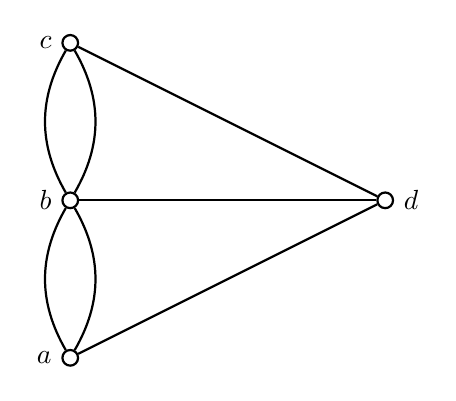
\begin{tikzpicture}
[nodedecorate/.style={shape=circle,inner sep=2pt,draw,thick},%
  linedecorate/.style={-,thick}]
%% nodes or vertices
\foreach \nodename/\x/\y in {a/0/0, b/0/2, c/0/4, d/4/2} {
  \node (\nodename) at (\x,\y) [nodedecorate] {};
}
\foreach \nodename/\direction/\navigate in {a/left/west, b/left/west,
  c/left/west} {
  \node [\direction] at (\nodename.\navigate) {$\nodename$};
}
\node [right] at (d.east) {$d$};
%% edges or lines
\path
\foreach \startnode/\endnode in {a/d, b/d, c/d} {
  (\startnode) edge[linedecorate] node {} (\endnode)
};
\path
\foreach \startnode/\endnode in {a/b, b/c} {
  (\startnode) edge[linedecorate,bend left] node {} (\endnode)
};
\path
\foreach \startnode/\endnode in {c/b, b/a} {
  (\startnode) edge[linedecorate,bend left] node {} (\endnode)
};
\end{tikzpicture}
\caption{The seven bridges of K\"onigsberg puzzle.}
\label{fig:introduction:seven_bridges_Konigsberg}
\end{figure}


%%-----------------------------------------------------------------------%%
%%--- Graphs and digraphs -----------------------------------------------%%

\section{Graphs and digraphs}
\label{sec:introduction:graphs_digraphs}

To paraphrase what Felix Klein said about curves,\footnote{
``Everyone knows what a curve is, until he has studied enough
mathematics to become confused through the countless number of
possible exceptions.''}
it is easy to define a graph until you realize the countless number of
exceptions. There are directed graphs, weighted graphs, multigraphs,
simple graphs, and so on. Where do we begin?
\index{Klein, Felix}

We start by calling a ``graph'' what some call an ``unweighted,
undirected graph without multiple edges.'' A \emph{graph}\index{graph}
$G = (V, E)$ is an ordered pair of sets. Elements of $V$ are called
\emph{vertices}\index{vertices} or \emph{nodes}, and elements of
$E \subseteq V \times V$ are called \emph{edges}\index{edges} or
\emph{arcs}. We refer to $V$ as the vertex set of $G$, with $E$ being
the edge set. The cardinality of $V$ is called the
\emph{order}\index{order} of $G$, and $|E|$ is called the
\emph{size}\index{size} of $G$. We usually disregard any direction of
the edges and consider $(u,v)$ and $(v,u)$ as one and the same edge in
$G$. In that case, $G$ is referred to as an
\emph{undirected graph}\index{undirected graph}.

One can label a graph by attaching labels to its vertices. If $(v_1,
v_2) \in E$ is an edge of a graph $G = (V, E)$, we say that $v_1$ and
$v_2$ are \emph{adjacent} vertices. For ease of notation, we write the
edge $(v_1, v_2)$ as $v_1 v_2$. The edge $v_1 v_2$ is also said to be
\emph{incident} with the vertices $v_1$ and $v_2$.
\index{edges!incident}
\index{vertices!adjacent}

\begin{figure}[!htbp]
\centering
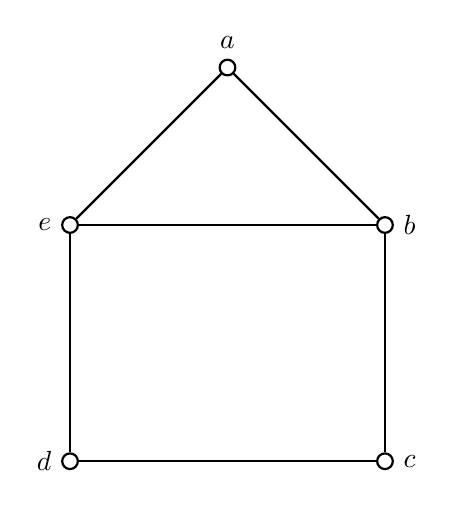
\begin{tikzpicture}
[nodedecorate/.style={shape=circle,inner sep=2pt,draw,thick},%
  linedecorate/.style={-,thick}]
%% nodes or vertices
\foreach \nodename/\x/\y/\direction/\navigate in {a/0/5/above/north,
  b/2/3/right/east, e/-2/3/left/west, c/2/0/right/east,
  d/-2/0/left/west} {
  \node (\nodename) at (\x,\y) [nodedecorate] {};
  \node [\direction] at (\nodename.\navigate) {$\nodename$};
}
%% edges or lines
\path
\foreach \startnode/\endnode in {a/b, b/c, b/e, c/d, d/e, e/a} {
  (\startnode) edge[linedecorate] node {} (\endnode)
};
\end{tikzpicture}
\caption{A house graph.}
\label{fig:introduction:house_graph}
\end{figure}
\index{house graph}

\begin{example}
\label{eg:introduction:house_graph}
Consider the graph in Figure~\ref{fig:introduction:house_graph}.
%
\begin{enumerate}
\item List the vertex and edge sets of the graph.

\item For each vertex, list all vertices that are adjacent to it.

\item Which vertex or vertices have the largest number of adjacent
  vertices? Similarly, which vertex or vertices have the smallest
  number of adjacent vertices?

\item If all edges of the graph are removed, is the resulting figure
  still a graph? Why or why not?

\item If all vertices of the graph are removed, is the resulting
  figure still a graph? Why or why not?
\end{enumerate}
\end{example}

\begin{proof}[Solution]
(1) Let $G = (V, E)$ denote the graph in
Figure~\ref{fig:introduction:house_graph}. Then the vertex set of $G$
is $V = \{ a, b, c, d, e \}$. The edge set of $G$ is given by
\begin{equation}
\label{eq:introduction:edges_of_house_graph}
E
=
\{ ab, ae, ba, bc, be, cb, cd, dc, de, ed, eb, ea \}.
\end{equation}
We can also use Sage to construct the graph $G$ and list its vertex
and edge sets:
%
\begin{center}
\fontsize{9pt}{9pt}
\selectfont
\tt
\begin{lstlisting}
sage: G = Graph({"a": ["b", "e"], "b": ["a", "c", "e"], "c": ["b", "d"], \
....: "d": ["c", "e"], "e": ["a", "b", "d"]})
sage: G
Graph on 5 vertices
sage: G.vertices()
['a', 'b', 'c', 'd', 'e']
sage: G.edges(labels=False)
[('a', 'b'), ('a', 'e'), ('b', 'e'), ('c', 'b'), ('c', 'd'), ('e', 'd')]
\end{lstlisting}
\end{center}
%
The graph $G$ is undirected, meaning that we do not impose direction
on any edges. Without any direction on the edges, the edge $ab$ is the
same as the edge $ba$. That is why \texttt{G.edges()} returns six
edges instead of the 12 edges listed
in~(\ref{eq:introduction:edges_of_house_graph}).

\index{$\adj$}
(2) Let $\adj(v)$ be the set of all vertices that are adjacent
to $v$. Then we have
%
\begin{align*}
\text{adj}(a) &= \{ b, e \} \\
\text{adj}(b) &= \{ a, c, e \} \\
\text{adj}(c) &= \{ b, d \} \\
\text{adj}(d) &= \{ c, e \} \\
\text{adj}(e) &= \{ a, b, d \}.
\end{align*}
%
The vertices adjacent to $v$ are also referred to as its
\emph{neighbors}. We can use the function \texttt{G.neighbors()} to
list all the neighbors of each vertex.
%
\begin{center}
\fontsize{9pt}{9pt}
\selectfont
\tt
\begin{lstlisting}
sage: G.neighbors("a")
['b', 'e']
sage: G.neighbors("b")
['a', 'c', 'e']
sage: G.neighbors("c")
['b', 'd']
sage: G.neighbors("d")
['c', 'e']
sage: G.neighbors("e")
['a', 'b', 'd']
\end{lstlisting}
\end{center}

(3) Taking the cardinalities of the above five sets, we get
$|\text{adj}(a)| = |\text{adj}(c)| = |\text{adj}(d)| = 2$ and
$|\text{adj}(b)| = |\text{adj}(e)| = 3$. Thus $a$, $c$ and $d$ have
the smallest number of adjacent vertices, while $b$ and $e$ have the
largest number of adjacent vertices.

(4) If all the edges in $G$ are removed, the result is still a graph,
although one without any edges. By definition, the edge set of any
graph is a subset of $V \times V$. Removing all edges of $G$ leaves us
with the empty set $\emptyset$, which is a subset of every set.

(5) Say we remove all of the vertices from the graph in
Figure~\ref{fig:introduction:house_graph} and in the process all edges
are removed as well. The result is that both of the vertex and edge
sets are empty. This is a special graph known as an \emph{empty} or
\emph{null} graph.
\end{proof}
\index{graph!null}
\index{null graph}

\begin{example}
Consider the illustration in
Figure~\ref{fig:introduction:self_loop}. Does
Figure~\ref{fig:introduction:self_loop} represent a graph? Why or why not?
\end{example}

\begin{proof}[Solution]
If $V = \{ a, b, c \}$ and $E = \{ aa, bc \}$, it is clear that $E
\subseteq V \times V$. Then $(V, E)$ is a graph. The edge $aa$ is
called a \emph{self-loop} of the graph. In general, any edge of the
form $vv$ is a self-loop.
\end{proof}
\index{self-loop}

\begin{figure}[!htbp]
\centering
\begin{tikzpicture}
[nodedecorate/.style={shape=circle,inner sep=2pt,draw,thick},%
  arrowdecorate/.style={-,thick}]
%% nodes or vertices
\foreach \nodename/\x/\y/\direction/\navigate in {c/-2/0/left/west,
  b/2/0/right/east, a/0/2/above/north} {
  \node (\nodename) at (\x,\y) [nodedecorate] {};
  \node [\direction] at (\nodename.\navigate) {$\nodename$};
}
%% edges or lines
\path
(a) edge[arrowdecorate,loop below,min distance=10mm,out=310,in=230] node {} (a)
(b) edge[arrowdecorate] node {} (c);
\end{tikzpicture}
\caption{A figure with a self-loop.}
\label{fig:introduction:self_loop}
\end{figure}

In Figure~\ref{fig:introduction:house_graph}, the edges $ae$ and $ea$
represent one and the same edge. If we do not consider the direction
of the edges in the graph of
Figure~\ref{fig:introduction:house_graph}, then the graph has six
edges. However, if the direction of each edge is taken into account,
then there are 12 edges as listed
in~(\ref{eq:introduction:edges_of_house_graph}). The following
definition captures the situation where the direction of the edges are
taken into account.

A \emph{directed edge} is an edge such that one vertex incident with it
is designated as the head vertex and the other incident vertex is
designated as the tail vertex. A directed edge $uv$ is said to be
directed from its tail $u$ to its head $v$. A \emph{directed graph} or
\emph{digraph} $G$ is a graph such that each of whose edges is
directed. The \emph{indegree} $\id(v)$ of a vertex $v \in V(G)$ counts
the number of edges such that $v$ is the head of those edges. The
\emph{outdegree} $\od(v)$ of a vertex $v \in V(G)$ is the number of
edges such that $v$ is the tail of those edges.
\index{graph!directed}
\index{digraph}
\index{directed edge}
\index{indegree}
\index{outdegree}
\index{$\id$}
\index{$\od$}

It is important to distinguish a graph $G$ as being directed or
undirected. If $G$ is undirected and $uv \in E(G)$, then $uv$ and $vu$
represent the same edge. In case $G$ is a digraph, then $uv$ and $vu$
are different directed edges. For a digraph $G = (V, E)$ and a vertex
$v \in V$, all the neighbors of $v$ in $G$ are contained in $\adj(v)$,
i.e. the set of all neighbors of $v$. Just as we distinguish between
indegree and outdegree for a vertex in a digraph, we also distinguish
between in-neighbors and out-neighbors. The set of \emph{in-neighbors}
$\iadj(v) \subseteq \adj(v)$ of $v \in V$ consists of all those
vertices that contribute to the indegree of $v$. Similarly, the set
of \emph{out-neighbors} $\oadj(v) \subseteq \adj(v)$ of $v \in V$ are
those vertices that contribute to the outdegree of $v$. Then
\[
\iadj(v) \cap \oadj(v)
=
\{u \;|\; uv \in E \text{ and } vu \in E\}
\]
and $\adj(v) = \iadj(v) \cup \oadj(v)$.
\index{$\iadj$}
\index{$\oadj$}
\index{in-neighbor}
\index{out-neighbor}

Another important class of graphs consist of those graphs having
multiple edges between pairs of vertices. A \emph{multigraph} is a
graph in which there are multiple edges between a pair of vertices. A
\emph{multi-undirected graph} is a multigraph that is
undirected. Similarly, a \emph{multidigraph} is a directed
multigraph.
\index{graph!multigraphs}
\index{multidigraph}
\index{multigraphs}
\index{multi-undirected graph}

The illustration in
Figure~\ref{fig:introduction:seven_bridges_Konigsberg} is actually a
multigraph called the K\"onigsberg graph. For a multigraph $G$, we are
given:
%
\begin{itemize}
\item A finite set $V$ whose elements are called \emph{vertices}.

\item A finite set $E$ whose elements are called \emph{edges}. We do
  not necessarily assume $E \subseteq V^{(2)}$, where $V^{(2)}$ is the
  set of unordered pairs of vertices.

\item An incidence function

\begin{equation}
\label{eqn:edge-incidence}
i: E \longrightarrow V^{(2)}.
\end{equation}
\end{itemize}
%
Such a multigraph is denoted $G = (V,E,i)$. An \emph{orientation} on
$G$ is a function
%
\begin{equation}
\label{eqn:edge-orientation}
h: E \longrightarrow V
\end{equation}
%
where $h(e) \in i(e)$ for all $e \in E$. The element $v = h(e)$ is
called the \emph{head} of $i(e)$. If $G$ has no self-loops, then
$i(e)$ is a set having exactly two elements denoted
$i(e) = \{h(e),\, t(e)\}$. The element $v = t(e)$ is called the
\emph{tail} of $i(e)$. For self-loops, we set $t(e) = h(e)$. A
multigraph with an orientation can therefore be described as the
$4$-tuple $(V, E, i, h)$. In other words, $G = (V,E,i,h)$ is a
multidigraph.
\index{orientation}
\index{edge!head}
\index{edge!tail}

\index{graph!simple}
\index{simple graph}
A \emph{simple graph} is a graph with no self-loops and no multiple
edges. Figure~\ref{fig:introduction:simple_graph_digraph_multidigraph}
illustrates a simple graph and its digraph version, together with a
multidigraph version of the K\"onigsberg graph. The edges of a digraph
can be visually represented as directed arrows, similar to the digraph
in
Figure~\ref{fig:introduction:triangle_digraph} and the multidigraph in
Figure~\ref{fig:introduction:Konigsberg_multidigraph}. The digraph in
Figure~\ref{fig:introduction:triangle_digraph} has the vertex set
$\{a, b, c\}$ and the edge set $\{ab, bc, ca\}$. There is an arrow
from vertex $a$ to vertex $b$, hence $ab$ is in the edge set. However,
there is no arrow from $b$ to $a$, so $ba$ is not in the edge set of
the graph in Figure~\ref{fig:introduction:triangle_digraph}. The
family $\Sh(n)$ of Shannon multigraphs is illustrated in
Figure~\ref{fig:introduction:Shannon_multigraphs} for integers
$2 \leq n \leq 7$. These graphs are named after Claude
E. Shannon~(1916--2001). Each Shannon multigraph consists of three
vertices, giving rise to a total of three distinct unordered
pairs. Two of these pairs are connected by $\lfloor n/2 \rfloor$
edges and the third pair of vertices is connected by
$\lfloor (n + 1) / 2 \rfloor$ edges.
\index{Shannon multigraphs}
\index{Shannon, Claude E.}

\begin{figure}[!htbp]
\centering
%%
%% simple graph
\subfigure[Simple graph.]{
\label{fig:introduction:triangle_simple_graph}
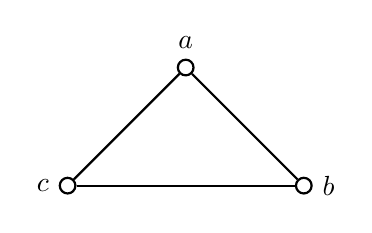
\begin{tikzpicture}
[nodedecorate/.style={shape=circle,inner sep=2pt,draw,thick},%
  linedecorate/.style={-,thick}]
%% nodes or vertices
\foreach \nodename/\x/\y/\direction/\navigate in {c/-1.5/0/left/west,
  b/1.5/0/right/east, a/0/1.5/above/north} {
  \node (\nodename) at (\x,\y) [nodedecorate] {};
  \node [\direction] at (\nodename.\navigate) {$\nodename$};
}
%% edges or lines
\path
\foreach \startnode/\endnode in {a/b, b/c, c/a} {
  (\startnode) edge[linedecorate] node {} (\endnode)
};
\end{tikzpicture}
}
\quad
%%
%% digraph
\subfigure[Digraph.]{
\label{fig:introduction:triangle_digraph}
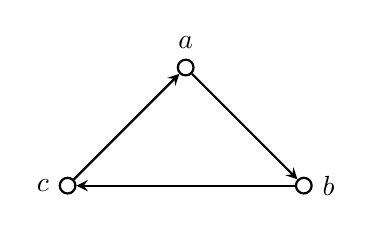
\begin{tikzpicture}
[nodedecorate/.style={shape=circle,inner sep=2pt,draw,thick},%
  arrowdecorate/.style={->,>=stealth,thick}]
%% nodes or vertices
\foreach \nodename/\x/\y/\direction/\navigate in {c/-1.5/0/left/west,
  b/1.5/0/right/east, a/0/1.5/above/north} {
  \node (\nodename) at (\x,\y) [nodedecorate] {};
  \node [\direction] at (\nodename.\navigate) {$\nodename$};
}
%% edges or lines
\path
\foreach \startnode/\endnode in {a/b, b/c, c/a} {
  (\startnode) edge[arrowdecorate] node {} (\endnode)
};
\end{tikzpicture}
}
\quad
%%
%% multidigraph
\subfigure[Multidigraph.]{
\label{fig:introduction:Konigsberg_multidigraph}
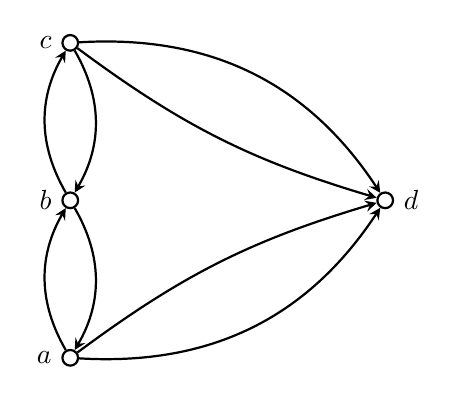
\begin{tikzpicture}
[nodedecorate/.style={shape=circle,inner sep=2pt,draw,thick},%
  arrowdecorate/.style={->,>=stealth,thick}]
%% nodes or vertices
\foreach \nodename/\x/\y in {a/0/0, b/0/2, c/0/4, d/4/2} {
  \node (\nodename) at (\x,\y) [nodedecorate] {};
}
\foreach \nodename/\direction/\navigate in {a/left/west, b/left/west,
  c/left/west} {
  \node [\direction] at (\nodename.\navigate) {$\nodename$};
}
\node [right] at (d.east) {$d$};
%% edges or lines
\path
\foreach \startnode/\endnode in {a/b, b/c} {
  (\startnode) edge[arrowdecorate,bend left] node {} (\endnode)
};
\path
\foreach \startnode/\endnode in {c/b, b/a} {
  (\startnode) edge[arrowdecorate,bend left] node {} (\endnode)
};
%% multiple directed edges
\path
(a) edge[arrowdecorate,bend left=10] node {} (d)
(c) edge[arrowdecorate,bend left] node {} (d)
(a) edge[arrowdecorate,bend right] node {} (d)
(c) edge[arrowdecorate,bend right=10] node {} (d);
\end{tikzpicture}
}
\caption{A simple graph, its digraph version, and a multidigraph.}
\label{fig:introduction:simple_graph_digraph_multidigraph}
\end{figure}

\begin{figure}[!htbp]
\centering
%%
%% Shannon multigraph Sh(2)
\subfigure[$\Sh(2)$]{
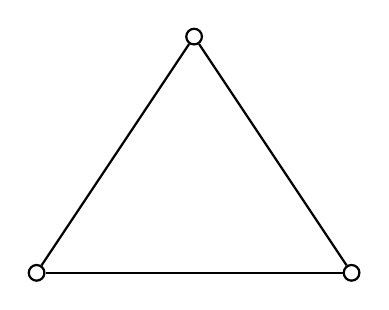
\begin{tikzpicture}
[nodedecorate/.style={shape=circle,inner sep=2pt,draw,thick},%
  linedecorate/.style={-,thick}]
%% nodes or vertices
\foreach \nodename/\x/\y in {a/-2/0, b/2/0, c/0/3} {
  \node (\nodename) at (\x,\y) [nodedecorate] {};
}
%% edges or lines
\path
\foreach \startnode/\endnode in {a/b, b/c, c/a} {
  (\startnode) edge[linedecorate] node {} (\endnode)
};
\end{tikzpicture}
}
\quad
%%
%% Shannon multigraph Sh(3)
\subfigure[$\Sh(3)$]{
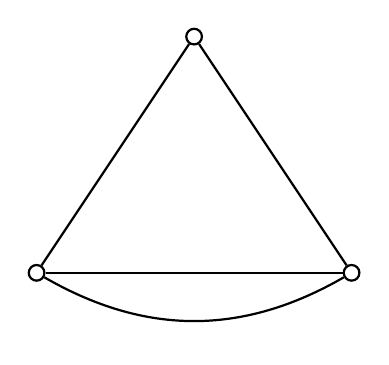
\begin{tikzpicture}
[nodedecorate/.style={shape=circle,inner sep=2pt,draw,thick},%
  linedecorate/.style={-,thick}]
%% nodes or vertices
\foreach \nodename/\x/\y in {a/-2/0, b/2/0, c/0/3} {
  \node (\nodename) at (\x,\y) [nodedecorate] {};
}
%% edges or lines
\path
\foreach \startnode/\endnode in {a/b, b/c, c/a} {
  (\startnode) edge[linedecorate] node {} (\endnode)
}
(a) edge[linedecorate,bend right] node {} (b);
\end{tikzpicture}
}
\quad
%%
%% Shannon multigraph Sh(4)
\subfigure[$\Sh(4)$]{
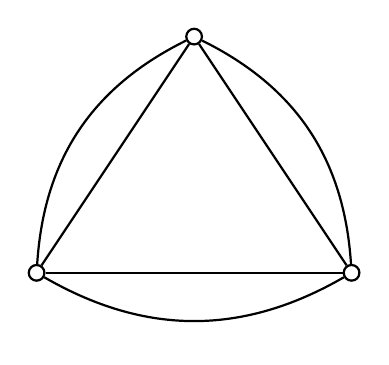
\begin{tikzpicture}
[nodedecorate/.style={shape=circle,inner sep=2pt,draw,thick},%
  linedecorate/.style={-,thick}]
%% nodes or vertices
\foreach \nodename/\x/\y in {a/-2/0, b/2/0, c/0/3} {
  \node (\nodename) at (\x,\y) [nodedecorate] {};
}
%% edges or lines
\path
\foreach \startnode/\endnode in {a/b, b/c, c/a} {
  (\startnode) edge[linedecorate] node {} (\endnode)
  (\startnode) edge[linedecorate,bend right] node {} (\endnode)
};
\end{tikzpicture}
}
%%
%% Shannon multigraph Sh(5)
\subfigure[$\Sh(5)$]{
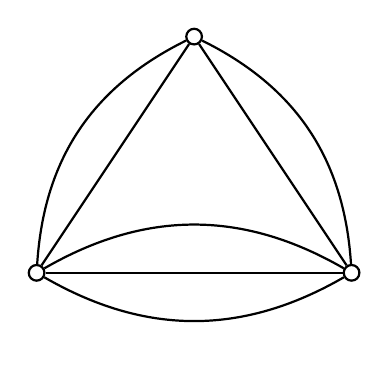
\begin{tikzpicture}
[nodedecorate/.style={shape=circle,inner sep=2pt,draw,thick},%
  linedecorate/.style={-,thick}]
%% nodes or vertices
\foreach \nodename/\x/\y in {a/-2/0, b/2/0, c/0/3} {
  \node (\nodename) at (\x,\y) [nodedecorate] {};
}
%% edges or lines
\path
\foreach \startnode/\endnode in {a/b, b/c, c/a} {
  (\startnode) edge[linedecorate] node {} (\endnode)
  (\startnode) edge[linedecorate,bend right] node {} (\endnode)
}
(a) edge[linedecorate,bend left] node {} (b);
\end{tikzpicture}
}
\quad
%%
%% Shannon multigraph Sh(6)
\subfigure[$\Sh(6)$]{
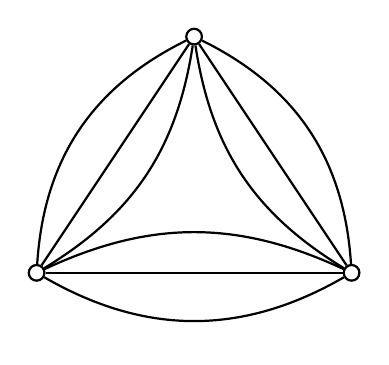
\begin{tikzpicture}
[nodedecorate/.style={shape=circle,inner sep=2pt,draw,thick},%
  linedecorate/.style={-,thick}]
%% nodes or vertices
\foreach \nodename/\x/\y in {a/-2/0, b/2/0, c/0/3} {
  \node (\nodename) at (\x,\y) [nodedecorate] {};
}
%% edges or lines
\path
\foreach \startnode/\endnode in {a/b, b/c, c/a} {
  (\startnode) edge[linedecorate] node {} (\endnode)
  (\startnode) edge[linedecorate,bend right] node {} (\endnode)
  (\startnode) edge[linedecorate,bend left=25] node {} (\endnode)
};
\end{tikzpicture}
}
\quad
%%
%% Shannon multigraph Sh(7)
\subfigure[$\Sh(7)$]{
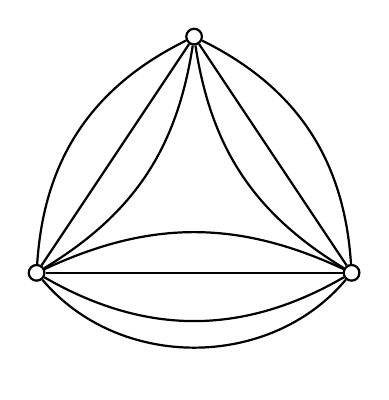
\begin{tikzpicture}
[nodedecorate/.style={shape=circle,inner sep=2pt,draw,thick},%
  linedecorate/.style={-,thick}]
%% nodes or vertices
\foreach \nodename/\x/\y in {a/-2/0, b/2/0, c/0/3} {
  \node (\nodename) at (\x,\y) [nodedecorate] {};
}
%% edges or lines
\path
\foreach \startnode/\endnode in {a/b, b/c, c/a} {
  (\startnode) edge[linedecorate] node {} (\endnode)
  (\startnode) edge[linedecorate,bend right] node {} (\endnode)
  (\startnode) edge[linedecorate,bend left=25] node {} (\endnode)
}
(a) edge[linedecorate,bend right=50] node {} (b);
\end{tikzpicture}
}
\caption{The family of Shannon multigraphs $\Sh(n)$ for $n = 1,\dots,7$.}
\label{fig:introduction:Shannon_multigraphs}
\end{figure}

For any vertex $v$ in a graph $G = (V, E)$, the cardinality of
$\text{adj}(v)$ is called the \emph{degree} of $v$ and written as
$\deg(v) = |\text{adj}(v)|$\index{$\deg$}. The degree of $v$ counts
the number of vertices in $G$ that are adjacent to $v$. If
$\deg(v) = 0$, we say that $v$ is an
\emph{isolated}\index{isolated vertex} vertex and if $\deg(v) = 1$
then $v$ is called a \emph{pendant}\index{pendant}. For example, in
the graph in Figure~\ref{fig:introduction:house_graph}, we have
$\deg(b) = 3$. For the graph in
Figure~\ref{fig:introduction:triangle_digraph}, we have
$\deg(b) = 2$. If $V \neq \emptyset$ and $E = \emptyset$, then
$G$ is a graph consisting entirely of isolated vertices. From
Example~\ref{eg:introduction:house_graph} we know that the vertices
$a, c, d$ in Figure~\ref{fig:introduction:house_graph} have the
smallest degree in the graph of that figure, while $b, e$ have the
largest degree. The minimum degree among all vertices in $G$ is
denoted $\delta(G)$, whereas the maximum degree is written as
$\Delta(G)$. Thus, if $G$ denotes the graph in
Figure~\ref{fig:introduction:house_graph} then we have $\delta(G) = 2$
and $\Delta(G) = 3$. In the following Sage session, we construct the
digraph in Figure~\ref{fig:introduction:triangle_digraph} and computes
its maximum and minimum number of degrees.
\index{$\delta$}
\index{$\Delta$}
\index{degree!maximum}
\index{degree!minimum}
\index{degree of a vertex}
\index{K\"onigsberg, seven bridges puzzle}
%
\begin{center}
\fontsize{9pt}{9pt}
\selectfont
\tt
\begin{lstlisting}
sage: G = DiGraph({"a": "b", "b": "c", "c": "a"})
sage: G
Digraph on 3 vertices
sage: G.degree("a")
2
sage: G.degree("b")
2
sage: G.degree("c")
2
\end{lstlisting}
\end{center}
%
So for the graph $G$ in
Figure~\ref{fig:introduction:simple_graph_digraph_multidigraph}, we have
$\delta(G) = \Delta(G) = 2$.

The graph $G$ in
Figure~\ref{fig:introduction:simple_graph_digraph_multidigraph}
has the special property that its minimum degree is the same as its
maximum degree, i.e. $\delta(G) = \Delta(G)$. Graphs with this
property are referred to as \emph{regular}. An $r$-\emph{regular}
graph is a regular graph each of whose vertices has degree $r$. For
instance, $G$ is a $2$-regular graph. The following result, due to
Euler, counts the total number of degrees in any graph.
\index{graph!regular}
\index{$r$-regular}
\index{regular graph}

\begin{theorem}
\label{thm:introduction:degree_sum}
\label{thm:introduction:hand_shaking}
\textbf{Euler 1736.}
If $G = (V, E)$ is a graph, then $\sum_{v \in V} \deg(v) = 2 |E|$.
\end{theorem}
\index{Euler, Leonhard}
\index{handshaking lemma}

\begin{proof}
Each edge $e = v_1 v_2 \in E$ is incident with two vertices, so $e$ is
counted twice towards the total sum of degrees. The first time, we
count $e$ towards the degree of vertex $v_1$ and the second time we
count $e$ towards the degree of $v_2$.
\end{proof}

Theorem~\ref{thm:introduction:hand_shaking} is sometimes called the
``handshaking lemma,'' due to its interpretation as in the following
story. Suppose you go into a room. Suppose there are $n$ people in the
room (including yourself) and some people shake hands with others and
some do not. Create the graph with $n$ vertices, where each vertex is
associated with a different person. Draw an edge between two people if
they shook hands. The degree of a vertex is the number of times that
person has shaken hands (we assume that there are no multiple edges,
i.e. that no two people shake hands twice). The theorem above simply
says that the total number of handshakes is even. This is ``obvious''
when you look at it this way since each handshake is counted twice
($A$ shaking $B$'s hand is counted, and $B$ shaking $A$'s hand is
counted as well, since the sum in the theorem is over all
vertices). To interpret Theorem~\ref{thm:introduction:hand_shaking} in
a slightly different way within the context of the same room of
people, there is an even number of people who shook hands with an odd
number of other people. This consequence of
Theorem~\ref{thm:introduction:hand_shaking} is recorded in the
following corollary.

\begin{corollary}
A graph $G = (V, E)$ contains an even number of vertices with odd
degrees.
\end{corollary}

\begin{proof}
Partition $V$ into two disjoint subsets: $V_e$ is the subset of $V$
that contains only vertices with even degrees; and $V_o$ is the subset
of $V$ with only vertices of odd degrees. That is, $V = V_e \cup V_o$
and $V_e \cap V_o = \emptyset$. From
Theorem~\ref{thm:introduction:hand_shaking}, we have
\[
\sum_{v \in V} \deg(v)
=
\sum_{v \in V_e} \deg(v) + \sum_{v \in V_o} \deg(v)
=
2 |E|
\]
which can be re-arranged as
\[
\sum_{v \in V_o} \deg(v)
=
\sum_{v \in V} \deg(v) - \sum_{v \in V_e} \deg(v).
\]
As $\sum_{v \in V} \deg(v)$ and $\sum_{v \in V_e} \deg(v)$ are both
even, their difference is also even.
\end{proof}

As $E \subseteq V \times V$, then $E$ can be the empty set, in which
case the total degree of $G = (V, E)$ is zero. Where $E \neq
\emptyset$, then the total degree of $G$ is greater than zero. By
Theorem~\ref{thm:introduction:degree_sum}, the total degree of $G$ is
non-negative and even. This result is an immediate consequence of
Theorem~\ref{thm:introduction:degree_sum} and is captured in the
following corollary.

\begin{corollary}
\label{cor:introduction:degree_sum_even}
If $G$ is a graph, then its total number of degrees is non-negative
and even.
\end{corollary}

If $G = (V, E)$ is an $r$-regular graph with $n$ vertices and $m$
edges, it is clear by definition of $r$-regular graphs that the total
degree of $G$ is $rn$. By Theorem~\ref{thm:introduction:degree_sum} we
have $2m = rn$ and therefore $m = rn / 2$. This result is captured in
the following corollary.

\begin{corollary}
If $G = (V, E)$ is an $r$-regular graph having $n$ vertices and $m$
edges, then $m = rn / 2$.
\end{corollary}


%%--- Problems ----------------------------------------------------------%%

\subsection*{Problems~\ref{sec:introduction:graphs_digraphs}}

\begin{enumerate}
\item Let $D = (V, E)$ be a digraph of size $q$. Show that
  \[
  \sum_{v \in V} \id(v)
  =
  \sum_{v \in V} \od(v)
  =
  q.
  \]
\end{enumerate}


%%-----------------------------------------------------------------------%%
%%--- Subgraphs and other graph types -----------------------------------%%

\section{Subgraphs and other graph types}
\label{sec:introduction:subgraphs_graph_types}

We now consider several common types of graphs. Along the way, we also
present basic properties of graphs that could be used to distinguish
different types of graphs.


%%--- Walks, trails, and paths ------------------------------------------%%

\subsection{Walks, trails, and paths}

If $u$ and $v$ are two vertices in a graph $G$, a $u$-$v$ \emph{walk}
is an alternating sequence of vertices and edges starting with $u$ and
ending at $v$. Consecutive vertices and edges are incident. Formally,
a walk $W$ of length $n \geq 0$ can be defined as
\[
W: v_0, e_1, v_1, e_2, v_2, \dots, v_{n-1}, e_n, v_n
\]
where each edge $e_i = v_{i-1} v_i$ and the length $n$ refers to the
number of~(not necessarily distinct) edges in the walk. The vertex
$v_0$ is the starting vertex of the walk and $v_n$ is the end vertex,
so we refer to $W$ as a $v_0$-$v_n$ walk. The \emph{trivial walk} is
the walk of length $n = 0$ in which the start and end vertices are one
and the same vertex. For brevity, we omit the edges in a walk and
usually write the walk as the following sequence of vertices:
\[
W: v_0, v_1, v_2, \dots, v_{n-1}, v_n.
\]
For the graph in Figure~\ref{fig:introduction:types_of_walks}, an
example of a walk is an $a$-$e$ walk: $a, b, c, b, e$. In other words,
we start at vertex $a$ and travel to vertex $b$. From $b$, we go to
$c$ and then back to $b$ again. Then we end our journey at $e$. Notice
that consecutive vertices in a walk are adjacent to each other. One
can think of vertices as destinations and edges as footpaths, say. We
are allowed to have repeated vertices and edges in a walk. The number
of edges in a walk is called its \emph{length}. For instance, the
walk $a, b, c, b, e$ has length $4$.
\index{walk}
\index{walk!length}

\begin{figure}[!htbp]
\centering
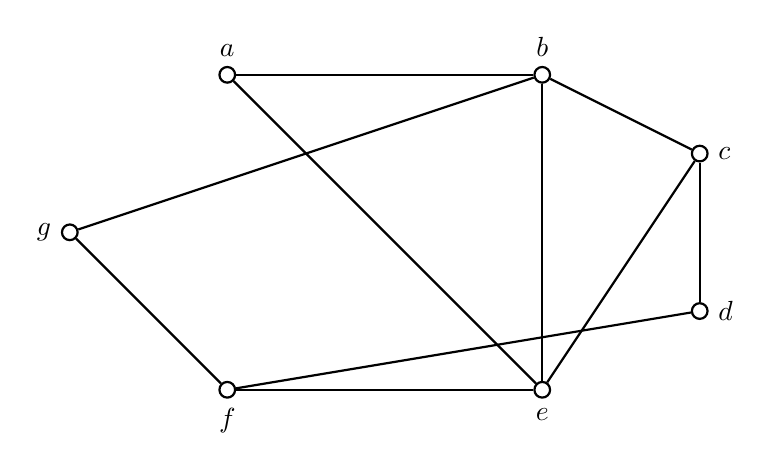
\begin{tikzpicture}
[nodedecorate/.style={shape=circle,inner sep=2pt,draw,thick},%
  linedecorate/.style={-,thick}]
%% nodes or vertices
\foreach \nodename/\x/\y/\direction/\navigate in {b/4/4/above/north,
  a/0/4/above/north, c/6/3/right/east, d/6/1/right/east,
  e/4/0/below/south, g/-2/2/left/west, f/0/0/below/south} {
  \node (\nodename) at (\x,\y) [nodedecorate] {};
  \node [\direction] at (\nodename.\navigate) {$\nodename$};
}
%% edges or lines
\path
\foreach \startnode/\endnode in {a/b, a/e, b/c, b/e, b/g, c/d, c/e,
  d/f, e/f, f/g} {
  (\startnode) edge[linedecorate] node {} (\endnode)
};
\end{tikzpicture}
\caption{Walking along a graph.}
\label{fig:introduction:types_of_walks}
\end{figure}

A \emph{trail} is a walk with no repeating edges. For example, the
$a$-$b$ walk $a, b, c, d, f, g, b$ in
Figure~\ref{fig:introduction:types_of_walks} is a trail. It does not
contain any repeated edges, but it contains one repeated vertex,
i.e. $b$. Nothing in the definition of a trail restricts a trail from
having repeated vertices.
A walk with no repeating vertices is called a \emph{path}. Without any
repeating vertices, a path cannot have repeating edges, hence a path
is also a trail.
\index{trail}
%\index{circuit}
\index{path}

\begin{corollary}
\label{cor:introduction:any_path_has_length_at_most_n_minus_1}
Let $G = (V, E)$ be a (di)graph of order $n = |V|$. Any path in $G$
has length at most $n - 1$.
\end{corollary}

\begin{proof}
Let $V = \{v_1, v_2, \dots, v_n\}$ be the vertex set of $G$. Without
loss of generality, we can assume that each pair of vertices in $G$ is
connected by an edge, giving a total of $n^2$ possible edges for
$E = V \times V$. We can remove self-loops from $E$, which now leaves
us with an edge set $E_1$ that consists of $n^2 - n$ edges. Start our
path from any vertex, say, $v_1$. To construct a path of length $1$,
choose an edge $v_1 v_{j_1} \in E_1$ such that
$v_{j_1} \notin \{v_1\}$. Remove from $E_1$ all $v_1 v_k$ such that
$v_{j_1} \neq v_k$. This results in a reduced edge set $E_2$ of
$n^2 - n - (n - 2)$ elements and we now have the path
$P_1: v_1, v_{j_1}$ of length $1$. Repeat the same process for
$v_{j_1} v_{j_2} \in E_2$ to obtain a reduced edge set $E_3$ of
$n^2 - n - 2(n - 2)$ elements and a path $P_2: v_1, v_{j_1}, v_{j_2}$
of length $2$. In general, let
$P_r: v_1, v_{j_1}, v_{j_2}, \dots, v_{j_r}$ be a path of length
$r < n$ and let $E_{r+1}$ be our reduced edge set of
$n^2 - n - r(n - 2)$ elements. Repeat the above process until we have
constructed a path
$P_{n-1}: v_1, v_{j_1}, v_{j_2}, \dots, v_{j_{n-1}}$ of length $n - 1$
with reduced edge set $E_n$ of $n^2 - n - (n - 1)(n - 2)$
elements. Adding another vertex to $P_{n-1}$ means going back to a
vertex that was previously visited, because $P_{n-1}$ already contains
all vertices of $V$.
\end{proof}

A path of length $n \geq 3$ whose start and end vertices are the same
is called a \emph{cycle}. For example, the walk $a, b, c, e, a$
in Figure~\ref{fig:introduction:types_of_walks} is a path and a cycle.
A walk which has no repeated edges and the start and end vertices are
the same, but otherwise has no  repeated vertices, is
%a \emph{circuit}, otherwise known as
a \emph{closed path}~(with apologies for slightly abusing
terminology).\footnote{
A closed path in a graph is sometimes also called a ``circuit.'' Since
that terminology unfortunately conflicts with the closely related
notion of a circuit of a matroid, we do not use it here.}
Thus the walk $a, b, e, a$ in
Figure~\ref{fig:introduction:types_of_walks} is a closed path. It is
easy to see that if you remove any edge from a cycle, then the
resulting walk contains no closed paths. An \emph{Euler subgraph} of a
graph $G$ is either a cycle or an edge-disjoint union of cycles in
$G$.
\index{closed path}
\index{cycle}
\index{path!closed}
\index{Euler subgraph}

The length of the shortest cycle in a graph is called the \emph{girth}
of the graph. An acyclic graph is said to have infinite girth, by
convention.
\index{girth}

\begin{example}
\label{eg:introduction:walks_paths_trails}
Consider the graph in Figure~\ref{fig:introduction:types_of_walks}.
%
\begin{enumerate}
\item Find two distinct walks that are not trails and determine their
  lengths.

\item Find two distinct trails that are not paths and determine their
  lengths.

\item Find two distinct paths and determine their lengths.

\item Find a closed path that is not a cycle.

\item Find a closed path $C$ which has an edge $e$ such that $C - e$
  contains a cycle.
\end{enumerate}
\end{example}

\begin{proof}[Solution]
(1) Here are two distinct walks that are not trails:
$w_1: g, b, e, a, b, e$ and $w_2: f, d, c, e, f, d$. The length of
walk $w_1$ is 5 and the length of walk $w_2$ is also 5.

(2) Here are two distinct trails that are not paths:
$t_1: a,b,c,e,b$ and $t_2: b,e,f,d,c,e$. The length of trail $t_1$ is
4 and the length of trail $t_2$ is 5.

(3) Here are two distinct paths: $p_1: a, b, c, d, f, e$ and
$p_2: g, b, a, e, f, d$. The length of path $p_1$ is 5 and the length
of path $p_2$ is also 5.

(4) Here is a closed path that is not a cycle: $d, c, e, b, a, e, f, d$.
\end{proof}

\begin{theorem}
\label{thm:introduction:every_walk_has_a_path}
Every $u$-$v$ walk in a graph contains a $u$-$v$ path.
\end{theorem}

\begin{proof}
A walk of length $n = 0$ is the trivial path. So assume that $W$ is a
$u$-$v$ walk of length $n > 0$ in a graph $G$:
\[
W: u = v_0, v_1, \dots, v_n = v.
\]
It is possible that a vertex in $W$ is assigned two different
labels. If $W$ has no repeated vertices, then $W$ is already a
path. Otherwise $W$ has at least one repeated vertex. Let
$0 \leq i,j \leq n$ be two distinct integers with $i < j$ such that
$v_i = v_j$. Deleting the vertices $v_i, v_{i+1}, \dots, v_{j-1}$ from
$W$ results in a $u$-$v$ walk $W_1$ whose length is less than $n$. If
$W_1$ is a path, then we are done. Otherwise we repeat the above
process to obtain a $u$-$v$ walk shorter than $W_1$. As $W$ is a
finite sequence, we only need to apply the above process a finite
number of times to arrive at a $u$-$v$ path.
\end{proof}

A graph is said to be \emph{connected} if for every pair of distinct
vertices $u, v$ there is a $u$-$v$ path joining them. A graph that is
not connected is referred to as \emph{disconnected}. The empty graph
is disconnected and so is any non-empty graph with an isolated
vertex. However, the graph in
Figure~\ref{fig:introduction:simple_graph_digraph_multidigraph} is
connected. A \emph{geodesic path} or \emph{shortest path} between two
distinct vertices $u,v$ of a graph is a $u$-$v$ path of minimum
length. A non-empty graph may have several shortest paths between some
distinct pair of vertices. For the graph in
Figure~\ref{fig:introduction:types_of_walks}, both $a,b,c$ and $a,e,c$
are geodesic paths between $a$ and $c$. The number of connected
components of a graph $G$ will be denoted $\omega(G)$.
\index{$\omega$}
\index{connected graph}
\index{disconnected graph}
\index{geodesic path}
\index{graph!connected}
\index{path!geodesic}
\index{shortest path}

\begin{example}
Determine whether or not the graph in
Figure~\ref{fig:introduction:types_of_walks} is connected. Find a
shortest path from $g$ to $d$.
\end{example}

\begin{proof}[Solution]
In the following Sage session, we first construct the graph in
Figure~\ref{fig:introduction:types_of_walks} and use the method
\verb!is_connected()! to determine whether or not the graph is
connected. Finally, we use the method \verb!shortest_path()! to find
a geodesic path between $g$ and $d$.
%
\begin{center}
\fontsize{9pt}{9pt}
\selectfont
\tt
\begin{lstlisting}
sage: g = Graph({"a": ["b", "e"], "b": ["a", "g", "e", "c"], \
....: "c": ["b", "e", "d"], "d": ["c", "f"], "e": ["f", "a", "b", "c"], \
....: "f": ["g", "d", "e"], "g": ["b", "f"]})
sage: g.is_connected()
True
sage: g.shortest_path("g", "d")
['g', 'f', 'd']
\end{lstlisting}
\end{center}
%
This shows that $g, f, d$ is a shortest path from $g$ to $d$. In fact,
any other $g$-$d$ path has length greater than $2$, so we can say that
$g, f, d$ is the shortest path between $g$ and $d$.
\end{proof}

We will explain Dijkstra's algorithm in
Chapter~\ref{chap:graph_algorithms}, which gives one of the best
algorithms for finding shortest paths between two vertices in a
connected graph. What is very remarkable is that, at the present state
of knowledge, finding the shortest path from a vertex $v$ to a
\emph{particular} (but arbitrarily given) vertex $w$ appears to be as
hard as finding the shortest path from a vertex $v$ to \emph{all}
other vertices in the graph!
\index{Dijkstra's algorithm}

Trees are a special type of graphs that are used in modelling
structures that have some form of hierarchy. For example, the
hierarchy within an organization can be drawn as a tree
structure, similar to the family tree in
Figure~\ref{fig:introduction:family_tree}. Formally, a \emph{tree} is
an undirected graph that is connected and has no cycles. If one vertex
of a tree is designated as the root vertex, then the tree is called a
\emph{rooted tree}. Chapter~\ref{chap:trees_forests} covers trees in
more details.
\index{family tree}
\index{tree}
\index{tree!rooted}

\begin{figure}[!htbp]
\centering
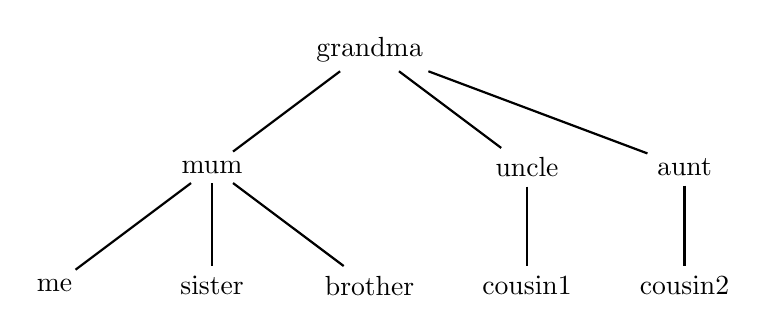
\begin{tikzpicture}
[nodedecorate/.style={shape=circle,inner sep=2pt,draw,thick},%
  linedecorate/.style={-,thick}]
%% nodes or vertices
\foreach \nodename/\x/\y in {me/0/0, sister/2/0, brother/4/0,
  mum/2/1.5, cousin1/6/0, cousin2/8/0, uncle/6/1.5, aunt/8/1.5,
  grandma/4/3} {
  \node (\nodename) at (\x,\y) [] {\nodename};
}
%% edges or lines
\path
\foreach \startnode/\endnode in {grandma/mum, grandma/uncle,
  grandma/aunt, mum/me, mum/sister, mum/brother, uncle/cousin1,
  aunt/cousin2} {
  (\startnode) edge[linedecorate] node {} (\endnode)
};
\end{tikzpicture}
\caption{A family tree.}
\label{fig:introduction:family_tree}
\end{figure}


%%--- Subgraphs, complete and bipartite graphs --------------------------%%

\subsection{Subgraphs, complete and bipartite graphs}

Let $G$ be a graph with vertex set $V(G)$ and edge set
$E(G)$. Consider a graph $H$ such that $V(H) \subseteq V(G)$ and $E(H)
\subseteq E(G)$. Furthermore, if $uv \in E(H)$ then $u,v \in
V(H)$. Then $H$ is called a \emph{subgraph} of $G$ and $G$ is referred
to as a \emph{supergraph} of $H$.
\index{subgraph}
\index{supergraph}

Starting from $G$, one can obtain its subgraph $H$ by deleting edges
and/or vertices from $G$. Note that when a vertex $v$ is removed from
$G$, then all edges incident with $v$ are also removed. If $V(H) =
V(G)$, then $H$ is called a \emph{spanning} subgraph of $G$. In
Figure~\ref{fig:introduction:star_subgraph}, let $G$ be the left-hand
side graph and let $H$ be the right-hand side graph. Then it is clear
that $H$ is a spanning subgraph of $G$. To obtain a spanning subgraph
from a given graph, we delete edges from the given graph.
\index{spanning subgraph}

\begin{figure}[!htbp]
\centering
%%
%% pentagon with star and inner pentagon
\subfigure[]{
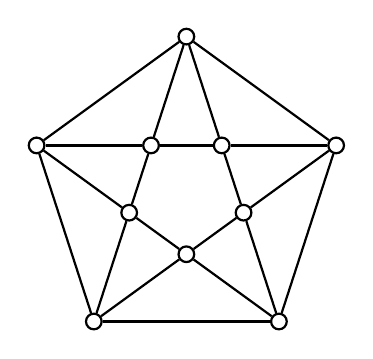
\begin{tikzpicture}
[nodedecorate/.style={shape=circle,inner sep=2pt,draw,thick},%
  linedecorate/.style={-,thick},%
  scale=2]
%% nodes or vertices
\foreach \nodename/\x/\y in {1/0.9510/0.3090, 2/0/1, 3/-0.9510/0.3090,
  4/-0.5877/-0.8090, 5/0.5877/-0.8090, 6/-0.2244/0.3090,
  7/0.2244/0.3090, 8/-0.3632/-0.1180, 9/0/-0.3819, 10/0.3632/-0.1180} {
  \node (\nodename) at (\x,\y) [nodedecorate] {};
}
%% edges or lines
\path
\foreach \startnode/\endnode in {1/2, 1/5, 1/7, 1/10, 2/3, 2/6, 2/7,
  3/4, 3/6, 3/8, 4/5, 4/8, 4/9, 5/9, 5/10, 6/7, 6/8, 7/10, 8/9, 9/10} {
  (\startnode) edge[linedecorate] node {} (\endnode)
};
\end{tikzpicture}
}
\qquad
%%
%% star and inner pentagon
\subfigure[]{
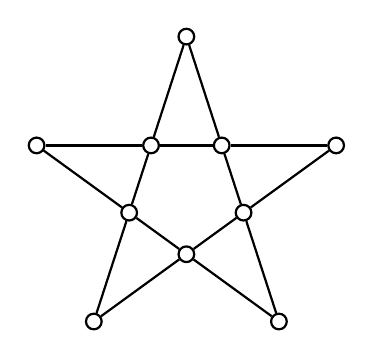
\begin{tikzpicture}
[nodedecorate/.style={shape=circle,inner sep=2pt,draw,thick},%
  linedecorate/.style={-,thick},%
  scale=2]
%% nodes or vertices
\foreach \nodename/\x/\y in {1/0.9510/0.3090, 2/0/1, 3/-0.9510/0.3090,
  4/-0.5877/-0.8090, 5/0.5877/-0.8090, 6/-0.2244/0.3090,
  7/0.2244/0.3090, 8/-0.3632/-0.1180, 9/0/-0.3819, 10/0.3632/-0.1180} {
  \node (\nodename) at (\x,\y) [nodedecorate] {};
}
%% edges or lines
\path
\foreach \startnode/\endnode in {1/7, 1/10, 2/6, 2/7, 3/6, 3/8, 4/8,
  4/9, 5/9, 5/10, 6/7, 6/8, 7/10, 8/9, 9/10} {
  (\startnode) edge[linedecorate] node {} (\endnode)
};
\end{tikzpicture}
}
\caption{A graph and one of its subgraphs.}
\label{fig:introduction:star_subgraph}
\end{figure}

\index{$K_n$}
\index{complete graph}
\index{graph!complete}
We now consider several standard classes of graphs. The \emph{complete}
graph $K_n$ on $n$ vertices is a graph such that any two distinct
vertices are adjacent. As $|V(K_n)| = n$, then $|E(K_n)|$ is
equivalent to the total number of 2-combinations from a set of $n$
objects:
%
\begin{equation}
\label{eq:introduction:size_of_K_n}
|E(K_n)|
=
\binom{n}{2}
=
\frac{n(n-1)}{2}.
\end{equation}
%
Thus for any graph $G$ with $n$ vertices, its total number of edges
$|E(G)|$ is bounded above by
\[
|E(G)|
\leq
\frac{n(n - 1)}{2}.
\]
Figure~\ref{fig:introduction:five_complete_graphs} shows complete
graphs each of whose total number of vertices is bounded by
$1 \leq n \leq 5$. The complete graph $K_1$ has one vertex with
no edges. It is also called the \emph{trivial} graph.
\index{graph!trivial}
\index{trivial graph}

\begin{figure}[!htbp]
\centering
%%
%% complete graph K_5
\subfigure[$K_5$]{
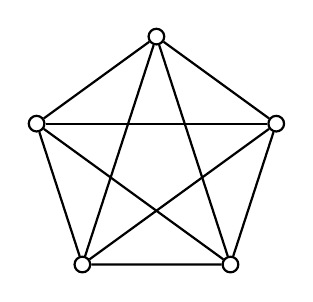
\begin{tikzpicture}
[nodedecorate/.style={shape=circle,inner sep=2pt,draw,thick},%
  linedecorate/.style={-,thick},%
  scale=1.6]
%% nodes or vertices
\foreach \nodename/\x/\y in {1/0.9510/0.3090, 2/0/1, 3/-0.9510/0.3090,
  4/-0.5877/-0.8090, 5/0.5877/-0.8090} {
  \node (\nodename) at (\x,\y) [nodedecorate] {};
}
%% edges or lines
\path
\foreach \startnode/\endnode in {1/2, 1/3, 1/4, 1/5, 2/3, 2/4, 2/5,
  3/4, 3/5, 4/5} {
  (\startnode) edge[linedecorate] node {} (\endnode)
};
\end{tikzpicture}
}
\quad
%%
%% complete graph K_4
\subfigure[$K_4$]{
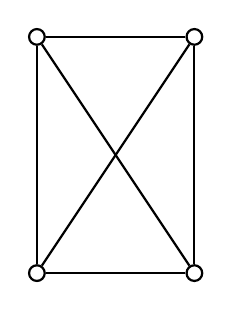
\begin{tikzpicture}
[nodedecorate/.style={shape=circle,inner sep=2pt,draw,thick},%
  linedecorate/.style={-,thick}]
%% nodes or vertices
\foreach \nodename/\x/\y in {1/0/0, 2/2/0, 3/2/3, 4/0/3} {
  \node (\nodename) at (\x,\y) [nodedecorate] {};
}
%% edges or lines
\path
\foreach \startnode/\endnode in {1/1, 1/2, 1/3, 1/4, 2/3, 2/4, 3/4} {
  (\startnode) edge[linedecorate] node {} (\endnode)
};
\end{tikzpicture}
}
\quad
%%
%% complete graph K_3
\subfigure[$K_3$]{
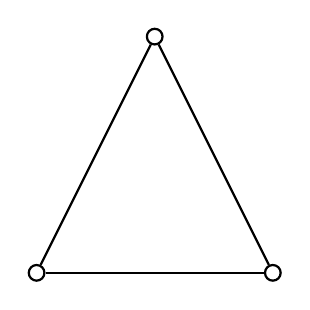
\begin{tikzpicture}
[nodedecorate/.style={shape=circle,inner sep=2pt,draw,thick},%
  linedecorate/.style={-,thick}]
%% nodes or vertices
\foreach \nodename/\x/\y in {1/0/0, 2/3/0, 3/1.5/3} {
  \node (\nodename) at (\x,\y) [nodedecorate] {};
}
%% edges or lines
\path
\foreach \startnode/\endnode in {1/2, 1/3, 2/3} {
  (\startnode) edge[linedecorate] node {} (\endnode)
};
\end{tikzpicture}
}
\quad
%%
%% complete graph K_2
\subfigure[$K_2$]{
\begin{tikzpicture}
[nodedecorate/.style={shape=circle,inner sep=2pt,draw,thick},%
  linedecorate/.style={-,thick}]
%% nodes or vertices
\node (1) at (0,0) [nodedecorate] {};
\node (2) at (0,3) [nodedecorate] {};
%% stub nodes that should not be visible
\node () at (-0.5,0) [] {};
\node () at (0.5,0) [] {};
%% edges or lines
\path
(1) edge[linedecorate] node {} (2);
\end{tikzpicture}
}
\quad
%%
%% complete graph K_1
\subfigure[$K_1$]{
\begin{tikzpicture}
[nodedecorate/.style={shape=circle,inner sep=2pt,draw,thick},%
  linedecorate/.style={-,thick}]
%% nodes or vertices
\node (1) at (0,0) [nodedecorate] {};
%% stub nodes that should not be visible
\node () at (-0.5,0) [] {};
\node () at (0.5,0) [] {};
\end{tikzpicture}
}
\caption{Complete graphs $K_n$ for $1 \leq n \leq 5$.}
\label{fig:introduction:five_complete_graphs}
\end{figure}

The \emph{cycle} graph on $n \geq 3$ vertices, denoted $C_n$, is the
connected $2$-regular graph on $n$ vertices. Each vertex in $C_n$ has
degree exactly $2$ and $C_n$ is
connected. Figure~\ref{fig:introduction:four_cycle_graphs} shows
cycles graphs $C_n$ where $3 \leq n \leq 6$. The \emph{path} graph on
$n \geq 1$ vertices is denoted $P_n$. For $n = 1, 2$ we have
$P_1 = K_1$ and $P_2 = K_2$. Where $n \geq 3$, then $P_n$ is a
spanning subgraph of $C_n$ obtained by deleting one edge.
\index{$C_n$}
\index{$P_n$}
\index{cycle graph}
\index{path graph}

\begin{figure}[!htbp]
\centering
%%
%% cycle graph C_6
\subfigure[$C_6$]{
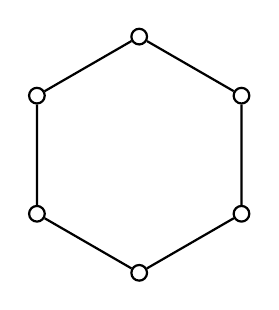
\begin{tikzpicture}
[nodedecorate/.style={shape=circle,inner sep=2pt,draw,thick},%
  linedecorate/.style={-,thick},%
  scale=1.5]
%% nodes or vertices
\foreach \nodename/\x/\y in {1/0.8660/0.5, 2/0/1, 3/-0.8660/0.5,
  4/-0.8660/-0.5, 5/0/-1, 6/0.8660/-0.5} {
  \node (\nodename) at (\x,\y) [nodedecorate] {};
}
%% edges or lines
\path
\foreach \startnode/\endnode in {1/2, 1/6, 2/3, 3/4, 4/5, 5/6} {
  (\startnode) edge[linedecorate] node {} (\endnode)
};
\end{tikzpicture}
}
\quad
%%
%% cycle graph C_5
\subfigure[$C_5$]{
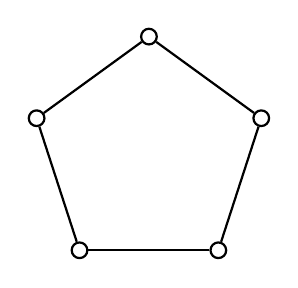
\begin{tikzpicture}
[nodedecorate/.style={shape=circle,inner sep=2pt,draw,thick},%
  linedecorate/.style={-,thick},%
  scale=1.5]
%% nodes or vertices
\foreach \nodename/\x/\y in {1/0.9510/0.3090, 2/0/1, 3/-0.9510/0.3090,
  4/-0.5877/-0.8090, 5/0.5877/-0.8090} {
  \node (\nodename) at (\x,\y) [nodedecorate] {};
}
%% edges or lines
\path
\foreach \startnode/\endnode in {1/2, 1/5, 2/3, 3/4, 4/5} {
  (\startnode) edge[linedecorate] node {} (\endnode)
};
\end{tikzpicture}
}
\quad
%%
%% cycle graph C_4
\subfigure[$C_4$]{
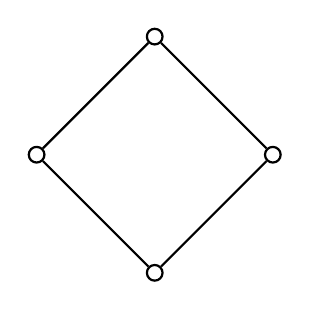
\begin{tikzpicture}
[nodedecorate/.style={shape=circle,inner sep=2pt,draw,thick},%
  linedecorate/.style={-,thick},%
  scale=1.5]
%% nodes or vertices
\foreach \nodename/\x/\y in {1/1/0, 2/0/1, 3/-1/0, 4/0/-1} {
  \node (\nodename) at (\x,\y) [nodedecorate] {};
}
%% edges or lines
\path
\foreach \startnode/\endnode in {1/2, 1/4, 2/3, 3/4} {
  (\startnode) edge[linedecorate] node {} (\endnode)
};
\end{tikzpicture}
}
\quad
%%
%% cycle graph C_3
\subfigure[$C_3$]{
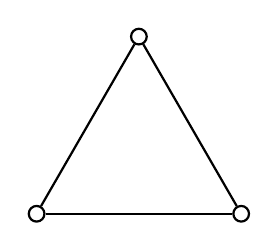
\begin{tikzpicture}
[nodedecorate/.style={shape=circle,inner sep=2pt,draw,thick},%
  linedecorate/.style={-,thick},%
  scale=1.5]
%% nodes or vertices
\foreach \nodename/\x/\y in {1/0.8660/-0.5, 2/0/1, 3/-0.8660/-0.5} {
  \node (\nodename) at (\x,\y) [nodedecorate] {};
}
%% edges or lines
\path
\foreach \startnode/\endnode in {1/2, 1/3, 2/3} {
  (\startnode) edge[linedecorate] node {} (\endnode)
};
\end{tikzpicture}
}
\caption{Cycle graphs $C_n$ for $3 \leq n \leq 6$.}
\label{fig:introduction:four_cycle_graphs}
\end{figure}

A \emph{bipartite} graph $G$ is a graph with at least two
vertices such that $V(G)$ can be split into two disjoint subsets $V_1$
and $V_2$, both non-empty. Every edge $uv \in E(G)$ is such that
$u \in V_1$ and $v \in V_2$, or $v \in V_1$ and $u \in V_2$.

The \emph{complete bipartite} graph $K_{m,n}$ is the bipartite graph
whose vertex set is partitioned into two non-empty disjoint sets $V_1$
and $V_2$ with $|V_1| = m$ and $|V_2| = n$. Any vertex in $V_1$ is
adjacent to each vertex in $V_2$, and any two distinct vertices in
$V_i$ are not adjacent to each other. If $m = n$, then $K_{n,n}$ is
$n$-regular. Where $m = 1$ then $K_{1,n}$ is called the \emph{star}
graph. Figure~\ref{fig:introduction:bipartite_complete_bipartite_graphs}
shows a bipartite graph together with the complete bipartite graphs
$K_{4,3}$ and $K_{3,3}$, and the star graph $K_{1,4}$.
\index{$K_{m,n}$}
\index{bipartite graph}
\index{complete bipartite graph}
\index{graph!bipartite}
\index{graph!complete bipartite}
\index{graph!star}
\index{star graph}

\begin{figure}[!htbp]
\centering
%%
%% bipartite graph
\subfigure[Bipartite]{
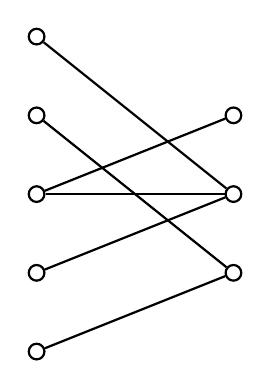
\begin{tikzpicture}
[nodedecorate/.style={shape=circle,inner sep=2pt,draw,thick},%
  linedecorate/.style={-,thick}]
%% nodes or vertices
\foreach \nodename/\x/\y in {a/0/0, b/0/1, c/0/2, d/0/3, e/0/4,
  f/2.5/3, g/2.5/2, h/2.5/1} {
  \node (\nodename) at (\x,\y) [nodedecorate] {};
}
%% edges or lines
\path
\foreach \startnode/\endnode in {a/h, b/g, c/g, c/f, d/h, e/g} {
  (\startnode) edge[linedecorate] node {} (\endnode)
};
\end{tikzpicture}
}
\quad
%%
%% complete bipartite graph K_{4,3}
\subfigure[$K_{4,3}$]{
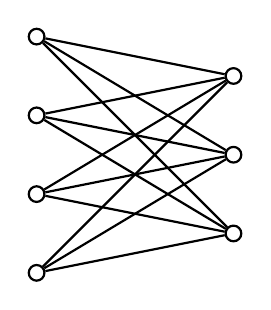
\begin{tikzpicture}
[nodedecorate/.style={shape=circle,inner sep=2pt,draw,thick},%
  linedecorate/.style={-,thick}]
%% nodes or vertices
\foreach \nodename/\x/\y in {a/0/0, b/0/1, c/0/2, d/0/3, e/2.5/2.5,
  f/2.5/1.5, g/2.5/0.5} {
  \node (\nodename) at (\x,\y) [nodedecorate] {};
}
%% edges or lines
\path
\foreach \startnode/\endnode in {a/e, a/f, a/g, b/e, b/f, b/g, c/e,
  c/f, c/g, d/e, d/f, d/g} {
  (\startnode) edge[linedecorate] node {} (\endnode)
};
\end{tikzpicture}
}
\quad
%%
%% complete bipartite graph K_{3,3}
\subfigure[$K_{3,3}$]{
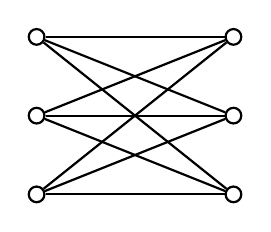
\begin{tikzpicture}
[nodedecorate/.style={shape=circle,inner sep=2pt,draw,thick},%
  linedecorate/.style={-,thick}]
%% nodes or vertices
\foreach \nodename/\x/\y in {a/0/0, b/0/1, c/0/2, d/2.5/2, e/2.5/1,
  f/2.5/0} {
  \node (\nodename) at (\x,\y) [nodedecorate] {};
}
%% edges or lines
\path
\foreach \startnode/\endnode in {a/d, a/e, a/f, b/d, b/e, b/f, c/d,
  c/e, c/f} {
  (\startnode) edge[linedecorate] node {} (\endnode)
};
\end{tikzpicture}
}
\quad
%%
%% star graph K_{1,4}
\subfigure[$K_{1,4}$]{
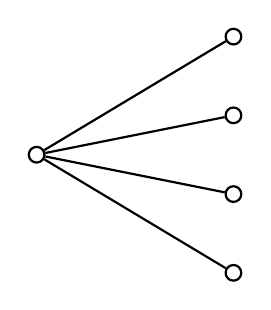
\begin{tikzpicture}
[nodedecorate/.style={shape=circle,inner sep=2pt,draw,thick},%
  linedecorate/.style={-,thick}]
%% nodes or vertices
\foreach \nodename/\x/\y in {a/0/1.5, b/2.5/3, c/2.5/2, d/2.5/1,
  e/2.5/0} {
  \node (\nodename) at (\x,\y) [nodedecorate] {};
}
%% edges or lines
\path
\foreach \startnode/\endnode in {a/b, a/c, a/d, a/e} {
  (\startnode) edge[linedecorate] node {} (\endnode)
};
\end{tikzpicture}
}
\caption{Bipartite, complete bipartite, and star graphs.}
\label{fig:introduction:bipartite_complete_bipartite_graphs}
\end{figure}

As an example of $K_{3,3}$, suppose that there are $3$ boys and $3$
girls dancing in a room. The boys and girls naturally partition the
set of all people in the room. Construct a graph having $6$ vertices,
each vertex corresponding to a person in the room, and draw an edge
form one vertex to another if the two people dance together. If each
girl dances three times, once with with each of the three boys, then
the resulting graph is $K_{3,3}$.

%%--- Problems ----------------------------------------------------------%%

\subsection*{Problems~\ref{sec:introduction:subgraphs_graph_types}}

\begin{enumerate}
\item If $G$ is a simple graph of order $n > 0$, show that
  $\deg(v) < n$ for all $v \in V(G)$.

\item Let $G$ be a graph of order $n$ and size $m$. Then $G$ is called
  an \emph{overfull graph} if
  $m > \Delta(G) \cdot \left\lfloor n / 2 \right\rfloor$. If
  $m = \Delta(G) \cdot \left\lfloor n / 2 \right\rfloor + 1$, then $G$
  is said to be \emph{just overfull}. It can be shown that overfull
  graphs have odd order. Equivalently, let $G$ be of odd order. We can
  define $G$ to be overfull if $m > \Delta(G) \cdot (n-1)/2$,
  and $G$ is just overfull if $m = \Delta(G) \cdot (n-1)/2 + 1$. Find
  an overfull graph and a graph that is just overfull.
\end{enumerate}


%%-----------------------------------------------------------------------%%
%%--- Representing graphs as matrices -----------------------------------%%

\section{Representing graphs using matrices}
\label{sec:introduction:matrix_representation}

An $m \times n$ matrix $A$ can be represented as
\[
A
=
\begin{bmatrix}
a_{11} & a_{12} & \cdots & a_{1n} \\
a_{21} & a_{22} & \cdots & a_{2n} \\
\hdotsfor{4} \\
a_{m1} & a_{m2} & \cdots & a_{mn} \\
\end{bmatrix}.
\]
The positive integers $m$ and $n$ are the row and column dimensions of
$A$, respectively. The entry in row $i$ column $j$ is denoted
$a_{ij}$. Where the dimensions of $A$ are clear from context, $A$ is
also written as $A = [a_{ij}]$.
\index{matrix}

Representing a graph as a matrix is very inefficient in some cases and
not so in other cases. Imagine you walk into a large room full of
people and you consider the ``handshaking graph'' discussed in
connection with Theorem~\ref{thm:introduction:hand_shaking}. If not
many people shake hands in the room, it is a waste of time recording
all the handshakes and also all the ``non-handshakes.'' This is
basically what the adjacency matrix does. In this kind of
``sparse graph'' situation, it would be much easier to simply record
the handshakes as a Python dictionary. This section requires some
concepts and techniques from linear algebra, especially matrix
theory. See introductory texts on linear algebra and matrix
theory~\cite{Beezer2009} for coverage of such concepts and techniques.


%%--- Adjacency matrix --------------------------------------------------%%

\subsection{Adjacency matrix}

Let $G$ be an undirected graph with vertices
$V = \{ v_1, \dots, v_n \}$ and edge set $E$. The
\emph{adjacency matrix} of $G$ is the $n \times n$ matrix
$A = [a_{ij}]$ defined by
\[
a_{ij}
=
\begin{cases}
1, & \text{if $v_i v_j \in E$}, \\
0, & \text{otherwise}.
\end{cases}
\]
As $G$ is an undirected graph, then $A$ is a symmetric matrix. That
is, $A$ is a square matrix such that $a_{ij} = a_{ji}$.

Now let $G$ be a directed graph with vertices
$V = \{ v_1, \dots, v_n \}$ and edge set $E$. The
$(0, -1, 1)$-\emph{adjacency matrix} of $G$ is the $n \times n$ matrix
$A = [a_{ij}]$ defined by
\index{adjacency matrix}
\[
a_{ij}
=
\begin{cases}
1,  & \text{if $v_i v_j \in E$}, \\
-1, & \text{if $v_j v_i \in E$}, \\
0,  & \text{otherwise}.
\end{cases}
\]

\begin{figure}[!htbp]
\centering
%%
%% digraph
\subfigure[]{
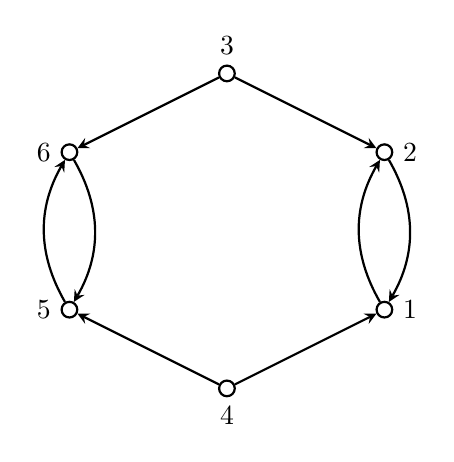
\begin{tikzpicture}
[nodedecorate/.style={shape=circle,inner sep=2pt,draw,thick},%
  arrowdecorate/.style={->,>=stealth,thick},%
  linedecorate/.style={-,thick}]
%% nodes or vertices
\foreach \nodename/\x/\y/\direction/\navigate in {1/2/1/right/east,
  2/2/3/right/east, 3/0/4/above/north, 4/0/0/below/south,
  5/-2/1/left/west, 6/-2/3/left/west} {
  \node (\nodename) at (\x,\y) [nodedecorate] {};
  \node [\direction] at (\nodename.\navigate) {$\nodename$};
}
%% edges or lines
\path
(1) edge[arrowdecorate,bend left] node {} (2)
(2) edge[arrowdecorate,bend left] node {} (1)
(3) edge[arrowdecorate] node {} (2)
(3) edge[arrowdecorate] node {} (6)
(4) edge[arrowdecorate] node {} (1)
(4) edge[arrowdecorate] node {} (5)
(5) edge[arrowdecorate,bend left] node {} (6)
(6) edge[arrowdecorate,bend left] node {} (5);
\end{tikzpicture}
}
\quad
%%
%% graph
\subfigure[]{
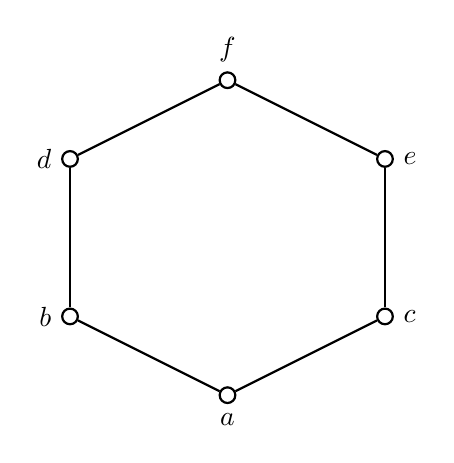
\begin{tikzpicture}
[nodedecorate/.style={shape=circle,inner sep=2pt,draw,thick},%
  linedecorate/.style={-,thick}]
%% nodes or vertices
\foreach \nodename/\x/\y/\direction/\navigate in {c/2/1/right/east,
  e/2/3/right/east, f/0/4/above/north, a/0/0/below/south,
  b/-2/1/left/west, d/-2/3/left/west} {
  \node (\nodename) at (\x,\y) [nodedecorate] {};
  \node [\direction] at (\nodename.\navigate) {$\nodename$};
}
%% edges or lines
\path
\foreach \startnode/\endnode in {c/e, c/a, e/f, f/d, a/b, b/d} {
  (\startnode) edge[linedecorate] node {} (\endnode)
};
\end{tikzpicture}
}
\caption{Adjacency matrices of directed and undirected graphs.}
\label{fig:introduction:adjacency_matrices}
\end{figure}

\begin{example}
Compute the adjacency matrices of the graphs in
Figure~\ref{fig:introduction:adjacency_matrices}.
\end{example}

\begin{proof}[Solution]
Define the graphs in Figure~\ref{fig:introduction:adjacency_matrices}
using \verb!DiGraph! and \verb!Graph!. Then call the method
\verb!adjacency_matrix()!.
%
\begin{center}
\fontsize{9pt}{9pt}
\selectfont
\tt
\begin{lstlisting}
sage: G1 = DiGraph({1: [2], 2: [1], 3: [2, 6], 4: [1, 5], 5: [6], 6: [5]})
sage: G2 = Graph({"a": ["b", "c"], "b": ["a", "d"], "c": ["a", "e"], \
....: "d": ["b", "f"], "e": ["c", "f"], "f": ["d", "e"]})
sage: m1 = G1.adjacency_matrix(); m1
[0 1 0 0 0 0]
[1 0 0 0 0 0]
[0 1 0 0 0 1]
[1 0 0 0 1 0]
[0 0 0 0 0 1]
[0 0 0 0 1 0]
sage: m2 = G2.adjacency_matrix(); m2
[0 1 1 0 0 0]
[1 0 0 1 0 0]
[1 0 0 0 1 0]
[0 1 0 0 0 1]
[0 0 1 0 0 1]
[0 0 0 1 1 0]
sage: m1.is_symmetric()
False
sage: m2.is_symmetric()
True
\end{lstlisting}
\end{center}
%
In general, the adjacency matrix of a digraph is not symmetric, while
that of an undirected graph is symmetric.
\end{proof}

%% \begin{theorem}
%% Let $G$ be a graph of order $n$ and $\mathbf{A}$ the adjacency matrix
%% of $G$. For each positive integer $k$, the $i$-$j$ entry of
%% $\mathbf{A}^k$ counts the number of $v_i$-$v_j$ walks of length $k$.
%% \end{theorem}

More generally, if $G$ is an undirected multigraph with edge
$e_{ij} = v_i v_j$ having multiplicity $w_{ij}$, or a weighted
graph with edge $e_{ij} = v_i v_j$ having weight $w_{ij}$, then we
can define the (weighted) \emph{adjacency matrix} $A = [a_{ij}]$ by
\[
a_{ij}
=
\begin{cases}
w_{ij}, & \text{if $v_i v_j \in E$}, \\
0,      & \text{otherwise}.
\end{cases}
\]
For example, Sage allows you to easily compute a weighted adjacency
matrix.
%
\begin{center}
\fontsize{9pt}{9pt}
\selectfont
\tt
\begin{lstlisting}
sage: G = Graph(sparse=True, weighted=True)
sage: G.add_edges([(0,1,1), (1,2,2), (0,2,3), (0,3,4)])
sage: M = G.weighted_adjacency_matrix(); M
[0 1 3 4]
[1 0 2 0]
[3 2 0 0]
[4 0 0 0]
\end{lstlisting}
\end{center}


%%--- Bipartite case ----------------------------------------------------%%

\subsubsection{Bipartite case}

Suppose $G = (V, E)$ is an undirected bipartite graph and
$V = V_1 \cup V_2$ is the partition of the vertices into $n_1$
vertices in $V_1$ and $n_2$ vertices in $V_2$, so $|V| = n_1 + n_2$.
Then the adjacency matrix $A$ of $G$ can be realized as a block
diagonal matrix
$A
=
\begin{bmatrix}
A_1 & 0 \\
0 & A_2
\end{bmatrix}$,
where $A_1$ is an $n_1 \times n_2$ matrix and $A_2$ is an
$n_2 \times n_1$ matrix. Since $G$ is undirected, $A_2 = A_1^T$.
The matrix is called a \emph{reduced adjacency matrix} or a
\emph{bi-adjacency matrix} (the literature also uses
the terms ``transfer matrix'' or the ambiguous term
``adjacency matrix'').
\index{adjacency matrix!reduced}
\index{bi-adjacency matrix}


%%--- Tanner graphs -----------------------------------------------------%%

\subsubsection{Tanner graphs}

If $H$ is an $m \times n$ $(0,1)$-matrix, then the \emph{Tanner graph}
of $H$ is the bipartite graph $G = (V,E)$ whose set of vertices
$V = V_1 \cup V_2$ is partitioned into two sets: $V_1$ corresponding
to the $m$ rows of $H$ and $V_2$ corresponding to the $n$ columns of $H$.
For any $i,j$ with $1 \leq i \leq m$ and $1 \leq j \leq n$, there is
an edge $ij \in E$ if and only if the $(i,j)$-th entry of $H$ is
$1$. This matrix $H$ is sometimes called the
reduced adjacency matrix or the \emph{check matrix} of the Tanner
graph. Tanner graphs are used in the theory of error-correcting
codes. For example, Sage allows you to easily compute such a bipartite
graph from its matrix.
\index{check matrix}
\index{Tanner graph}
%
\begin{center}
\fontsize{9pt}{9pt}
\selectfont
\tt
\begin{lstlisting}
sage: H = Matrix([(1,1,1,0,0), (0,0,1,0,1), (1,0,0,1,1)])
sage: B = BipartiteGraph(H)
sage: B.reduced_adjacency_matrix()
[1 1 1 0 0]
[0 0 1 0 1]
[1 0 0 1 1]
sage: B.plot(graph_border=True)
\end{lstlisting}
\end{center}
%
The corresponding graph is similar to that in
Figure~\ref{fig:introduction:tanner_graph}.

\begin{figure}[!htbp]
\centering
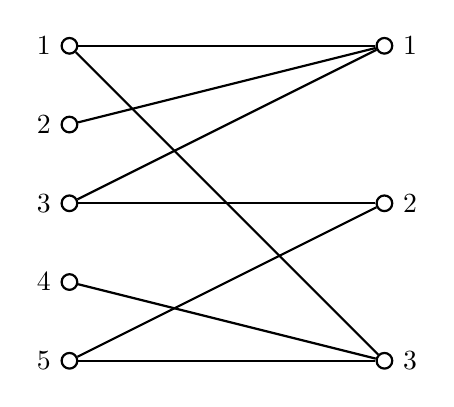
\begin{tikzpicture}
[nodedecorate/.style={shape=circle,inner sep=2pt,draw,thick},%
  linedecorate/.style={-,thick}]
%% nodes or vertices
\foreach \nodename/\nodelabel/\x/\y/\direction/\navigate in {
  c1/1/0/4/left/west, c2/2/0/3/left/west, c3/3/0/2/left/west,
  c4/4/0/1/left/west, c5/5/0/0/left/west, r1/1/4/4/right/east,
  r2/2/4/2/right/east, r3/3/4/0/right/east} {
  \node (\nodename) at (\x,\y) [nodedecorate] {};
  \node [\direction] at (\nodename.\navigate) {$\nodelabel$};
}
%% edges or lines
\path
\foreach \startnode/\endnode in {r1/c1, r1/c2, r1/c3, r2/c3, r2/c5,
  r3/c1, r3/c4, r3/c5} {
  (\startnode) edge[linedecorate] (\endnode)
};
\end{tikzpicture}
\caption{Tanner graph for $H$.}
\label{fig:introduction:tanner_graph}
\end{figure}

\begin{theorem}
Let $A$ be the adjacency matrix of a graph $G$ with vertex set
$V = \{v_1, v_2, \dots, v_p\}$. For each positive integer $n$, the
$ij$-th entry of $A^n$ counts the number of $v_i$-$v_j$ walks of
length $n$ in $G$.
\end{theorem}

\begin{proof}
We shall prove by induction on $n$. For the base case $n = 1$, the
$ij$-th entry of $A^1$ counts the number of walks of length 1 from
$v_i$ to $v_j$. This is obvious because $A^1$ is merely the adjacency
matrix $A$.

Suppose for induction that for some positive integer $k \geq 1$, the
$ij$-th entry of $A^k$ counts the number of walks of length $k$ from
$v_i$ to $v_j$. We need to show that the $ij$-th entry of $A^{k+1}$
counts the number of $v_i$-$v_j$ walks of length $k + 1$. Let
$A = [a_{ij}]$, $A^k = [b_{ij}]$, and $A^{k+1} = [c_{ij}]$. Since
$A^{k+1} = A A^k$, then
\[
c_{ij}
=
\sum_{r=1}^p a_{ir} b_{rj}
\]
for $i,j = 1, 2, \dots, p$. Note that $a_{ir}$ is the number of edges
from $v_i$ to $v_r$, and $b_{rj}$ is the number of $v_r$-$v_j$ walks
of length $k$. Any edge from $v_i$ to $v_r$ can be joined with any
$v_r$-$v_j$ walk to create a walk $v_i, v_r, \dots, v_j$ of length
$k + 1$. Then for each $r = 1, 2, \dots, p$, the value $a_{ir} b_{rj}$
counts the number of $v_i$-$v_j$ walks of length $k + 1$ with $v_r$
being the second vertex in the walk. Thus $c_{ij}$ counts the total
number of $v_i$-$v_j$ walks of length $k + 1$.
\end{proof}


%%--- Incidence matrix --------------------------------------------------%%

\subsection{Incidence matrix}

The relationship between edges and vertices provides a very strong
constraint on the data structure, much like the relationship between
points and blocks in a combinatorial design or points and lines in a
finite plane geometry. This incidence structure gives rise to another
way to describe a graph using a matrix.

Let $G$ be a digraph with edge set $E = \{ e_1, \dots, e_m \}$ and
vertex set $V = \{ v_1, \dots, v_n \}$. The \emph{incidence matrix} of
$G$ is the $n \times m$ matrix $B = [b_{ij}]$ defined by
\index{incidence matrix}
%
\begin{equation}
\label{eq:introduction:incidence_matrix_digraph}
b_{ij}
=
\begin{cases}
-1, & \text{if $v_i$ is the tail of $e_j$}, \\
1,  & \text{if $v_i$ is the head of $e_j$}, \\
2,  & \text{if $e_j$ is a self-loop at $v_i$}, \\
0,  & \text{otherwise}.
\end{cases}
\end{equation}
%
Each column of $B$ corresponds to an edge and each row corresponds to
a vertex. The definition of incidence matrix of a digraph as contained
in expression~(\ref{eq:introduction:incidence_matrix_digraph}) is
applicable to digraphs with self-loops as well as multidigraphs.

For the undirected case, let $G$ be an undirected graph with edge set
$E = \{ e_1, \dots, e_m \}$ and vertex set
$V = \{ v_1, \dots, v_n \}$. The \emph{unoriented incidence matrix} of
\index{incidence matrix!unoriented}
$G$ is the $n \times m$ matrix $B = [b_{ij}]$ defined by

\[
b_{ij}
=
\begin{cases}
1, & \text{if $v_i$ is incident to $e_j$}, \\
2, & \text{if $e_j$ is a self-loop at $v_i$}, \\
0, & \text{otherwise}.
\end{cases}
\]
An \emph{orientation} of an undirected graph $G$ is an assignment of
direction to each edge of $G$. The \emph{oriented incidence matrix} of
$G$ is defined similarly to the case where $G$ is a digraph: it is the
incidence matrix of any orientation of $G$. For each column of $B$, we
have $1$ as an entry in the row corresponding to one vertex of the
edge under consideration and $-1$ as an entry in the row corresponding
to the other vertex. Similarly, $b_{ij} = 2$ if $e_j$ is a self-loop
at $v_i$.
\index{orientation}
\index{oriented incidence matrix}
\index{incidence matrix!oriented}

%% Sage allows you to compute the incidence matrix of a
%% graph:
%% %\begin{example}
%% %
%% \begin{center}
%% \fontsize{9pt}{9pt}
%% \selectfont
%% \tt
%% \begin{lstlisting}
%% sage: G = Graph({1: [2, 4], 2: [1, 3], 3: [2, 6], 4: [1, 5], 5: [4, 6], 6: [3, 5]})
%% sage: G.incidence_matrix()
%% [-1 -1  0  0  0  0]
%% [ 0  1 -1  0  0  0]
%% [ 0  0  1 -1  0  0]
%% [ 1  0  0  0 -1  0]
%% [ 0  0  0  0  1 -1]
%% [ 0  0  0  1  0  1]
%% \end{lstlisting}
%% \end{center}
%
%\end{example}


%%--- Laplacian matrix --------------------------------------------------%%

\subsection{Laplacian matrix}

The \emph{degree matrix} of a graph $G = (V,E)$ is an $n \times n$
diagonal matrix $D$ whose $i$-th diagonal entry is the degree of the
$i$-th vertex in $V$. The \emph{Laplacian matrix} $\mathcal{L}$ of $G$
is the difference between the degree matrix and the adjacency matrix:
\[
\mathcal{L} = D - A.
\]
In other words, for an undirected unweighted simple graph,
$\mathcal{L} = [\ell_{ij}]$ is given by
\[
\ell_{ij}
=
\begin{cases}
-1,  & \text{if $i \neq j$ and $v_i v_j \in E$}, \\
d_i, & \text{if $i = j$}, \\
0,   & \text{otherwise},
\end{cases}
\]
where $d_i = \deg(v_i)$ is the degree of vertex $v_i$.
\index{$\mathcal{L}$}
\index{degree matrix}
\index{Laplacian matrix}

Sage allows you to compute the Laplacian matrix of a graph:
%
\begin{center}
\fontsize{9pt}{9pt}
\selectfont
\tt
\begin{lstlisting}
sage: G = Graph({1: [2,4], 2: [1,4], 3: [2,6], 4: [1,3], 5: [4,2], 6: [3,1]})
sage: G.laplacian_matrix()
[ 3 -1  0 -1  0 -1]
[-1  4 -1 -1 -1  0]
[ 0 -1  3 -1  0 -1]
[-1 -1 -1  4 -1  0]
[ 0 -1  0 -1  2  0]
[-1  0 -1  0  0  2]
\end{lstlisting}
\end{center}
%
There are many remarkable properties of the Laplacian matrix. It shall
be discussed further in Chapter~\ref{chap:distance_connectivity}.


%%--- Distance matrix ---------------------------------------------------%%

\subsection{Distance matrix}

\index{distance matrix}
Recall that the distance (or geodesic distance) $d(v,w)$ between two
vertices $v,w \in V$ in a connected graph $G = (V,E)$ is the number of
edges in a shortest path connecting them. The $n \times n$ matrix
$[d(v_i, v_j)]$ is the \emph{distance matrix} of $G$. Sage helps you
to compute the distance matrix of a graph:
%
\begin{center}
\fontsize{9pt}{9pt}
\selectfont
\tt
\begin{lstlisting}
sage: G = Graph({1: [2,4], 2: [1,4], 3: [2,6], 4: [1,3], 5: [4,2], 6: [3,1]})
sage: d = [[G.distance(i,j) for i in range(1,7)] for j in range(1,7)]
sage: matrix(d)
[0 1 2 1 2 1]
[1 0 1 1 1 2]
[2 1 0 1 2 1]
[1 1 1 0 1 2]
[2 1 2 1 0 3]
[1 2 1 2 3 0]
\end{lstlisting}
\end{center}

The distance matrix is an important quantity which allows one to
better understand the ``connectivity'' of a graph. Distance and
connectivity will be discussed in more detail in
Chapters~\ref{chap:distance_connectivity}
and~\ref{chap:random_graphs}.


%%--- Problems ----------------------------------------------------------%%

\subsection*{Problems~\ref{sec:introduction:matrix_representation}}

\begin{enumerate}
\item Let $G$ be an undirected graph whose unoriented incidence matrix
  is $M_u$ and whose oriented incidence matrix is $M_o$.
  \begin{enumerate}
  \item Show that the sum of the entries in any row of $M_u$ is the
    degree of the corresponding vertex.

  \item Show that the sum of the entries in any column of $M_u$ is
    equal to $2$.

  \item If $G$ has no self-loops, show that each column of $M_o$ sums
    to zero.
  \end{enumerate}

\item Let $G$ be a loopless digraph and let $M$ be its incidence
  matrix.
  \begin{enumerate}
  \item If $r$ is a row of $M$, show that the number of occurrences of
    $-1$ in $r$ counts the outdegree of the vertex corresponding to
    $r$. Show that the number of occurrences of $1$ in $r$ counts the
    indegree of the vertex corresponding to $r$.

  \item Show that each column of $M$ sums to $0$.
  \end{enumerate}

\item Let $G$ be a digraph and let $M$ be its incidence matrix. For
  any row $r$ of $M$, let $m$ be the frequency of $-1$ in $r$, let
  $p$ be the frequency of $1$ in $r$, and let $t$ be twice the
  frequency of $2$ in $r$. If $v$ is the vertex corresponding to
  $r$, show that the degree of $v$ is $\deg(v) = m + p + t$.
%%%%
%%%% Has ``the frequency'' been defined yet? American English
%%%% usage of this term might be different from Australian usage?
%%%%

\item Let $G$ be an undirected graph without self-loops and let $M$
  and its oriented incidence matrix. Show that the Laplacian matrix
  $\mathcal{L}$ of $G$ satisfies $\mathcal{L} = M \times M^T$, where
  $M^T$ is the transpose of $M$.
\end{enumerate}


%%-----------------------------------------------------------------------%%
%%--- Isomorphic graphs -------------------------------------------------%%

\section{Isomorphic graphs}
\label{chap:introduction:isomorphic_graphs}

Determining whether or not two graphs are, in some sense, the ``same''
is a hard but important problem. Two graphs $G$ and $H$ are
\emph{isomorphic} if there is a bijection
$f: V(G) \longrightarrow V(H)$ such that whenever $uv \in E(G)$ then
$f(u) f(v) \in E(H)$. The function $f$ is an \emph{isomorphism}
between $G$ and $H$. Otherwise, $G$ and $H$ are non-isomorphic. If
$G$ and $H$ are isomorphic, we write $G \cong H$.
\index{$\cong$}
\index{graph!isomorphic}
\index{graph isomorphism}

\begin{figure}[!htbp]
\centering
%%
%% cycle graph C_6
\subfigure[$C_6$]{
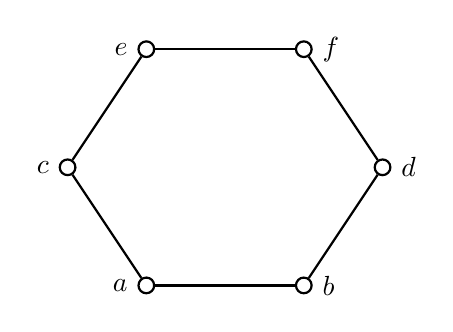
\begin{tikzpicture}
[nodedecorate/.style={shape=circle,inner sep=2pt,draw,thick},%
  linedecorate/.style={-,thick}]
%% nodes or vertices
\foreach \nodename/\x/\y/\direction/\navigate in {a/0/0/left/west,
  b/2/0/right/east, c/-1/1.5/left/west, d/3/1.5/right/east,
  e/0/3/left/west, f/2/3/right/east} {
  \node (\nodename) at (\x,\y) [nodedecorate] {};
  \node [\direction] at (\nodename.\navigate) {$\nodename$};
}
%% edges or lines
\path
\foreach \startnode/\endnode in {a/b, a/c, b/d, c/e, d/f, e/f} {
  (\startnode) edge[linedecorate] node {} (\endnode)
};
\end{tikzpicture}
}
%%
%% graph G_1 that is isomorphic to C_6
\subfigure[$G_1$]{
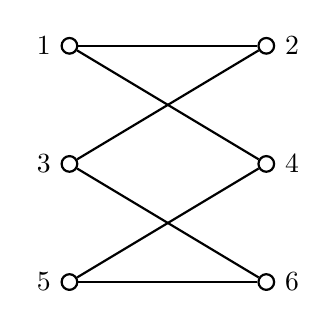
\begin{tikzpicture}
[nodedecorate/.style={shape=circle,inner sep=2pt,draw,thick},%
  linedecorate/.style={-,thick}]
%% nodes or vertices
\foreach \nodename/\x/\y/\direction/\navigate in {1/0/3/left/west,
  2/2.5/3/right/east, 3/0/1.5/left/west, 4/2.5/1.5/right/east,
  5/0/0/left/west, 6/2.5/0/right/east} {
  \node (\nodename) at (\x,\y) [nodedecorate] {};
  \node [\direction] at (\nodename.\navigate) {$\nodename$};
}
%% edges or lines
\path
\foreach \startnode/\endnode in {1/2, 1/4, 3/2, 3/6, 5/4, 5/6} {
  (\startnode) edge[linedecorate] node {} (\endnode)
};
\end{tikzpicture}
}
%%
%% graph G_2 that is non-isomorphic to C_6
\subfigure[$G_2$]{
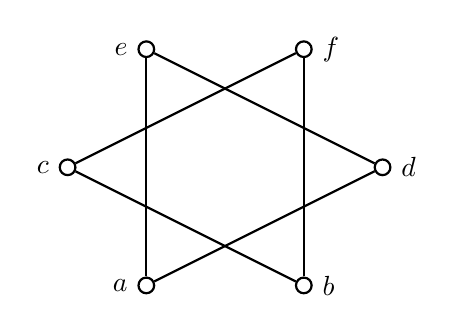
\begin{tikzpicture}
[nodedecorate/.style={shape=circle,inner sep=2pt,draw,thick},%
  linedecorate/.style={-,thick}]
%% nodes or vertices
\foreach \nodename/\x/\y/\direction/\navigate in {a/1/0/left/west,
  b/3/0/right/east, c/0/1.5/left/west, d/4/1.5/right/east,
  e/1/3/left/west, f/3/3/right/east} {
  \node (\nodename) at (\x,\y) [nodedecorate] {};
  \node [\direction] at (\nodename.\navigate) {$\nodename$};
}
%% edges or lines
\path
\foreach \startnode/\endnode in {a/d, a/e, b/c, b/f, c/f, d/e} {
  (\startnode) edge[linedecorate] node {} (\endnode)
};
\end{tikzpicture}
}
\caption{Isomorphic and non-isomorphic graphs.}
\label{fig:introduction:isomorphic_graphs}
\end{figure}

A graph $G$ is isomorphic to a graph $H$ if these two graphs can be
labelled in such a way that if $u$ and $v$ are adjacent in $G$, then
their counterparts in $V(H)$ are also adjacent in $H$. To determine
whether or not two graphs are isomorphic is to determine if they are
structurally equivalent. Graphs $G$ and $H$ may be drawn differently
so that they seem different. However, if $G \cong H$ then the
isomorphism $f: V(G) \longrightarrow V(H)$ shows that both of these
graphs are fundamentally the same. In particular, the order and size
of $G$ are equal to those of $H$, the isomorphism $f$ preserves
adjacencies, and $\deg(v) = \deg(f(v))$ for all $v \in G$. Since $f$
preserves adjacencies, then adjacencies along a given geodesic path
are preserved as well. That is, if $v_1, v_2, v_3, \dots, v_k$ is a
shortest path between $v_1, v_k \in V(G)$, then
$f(v_1), f(v_2), f(v_3), \dots, f(v_k)$ is a geodesic path between
$f(v_1), f(v_k) \in V(H)$.

\begin{example}
Consider the graphs in
Figure~\ref{fig:introduction:isomorphic_graphs}. Which pair of graphs
are isomorphic, and which two graphs are non-isomorphic?
\end{example}

\begin{proof}[Solution]
If \verb!G! is a Sage graph, one can use the method
\verb!G.is_isomorphic()! to determine whether or not the graph
\verb!G! is isomorphic to another graph. The following Sage session
illustrates how to use \verb!G.is_isomorphic()!.
%
\begin{center}
\fontsize{9pt}{9pt}
\selectfont
\tt
\begin{lstlisting}
sage: C6 = Graph({"a": ["b", "c"], "b": ["a", "d"], "c": ["a", "e"], \
....: "d": ["b", "f"], "e": ["c", "f"], "f": ["d", "e"]})
sage: G1 = Graph({1: [2, 4], 2: [1, 3], 3: [2, 6], 4: [1, 5], \
....: 5: [4, 6], 6: [3, 5]})
sage: G2 = Graph({"a": ["d", "e"], "b": ["c", "f"], "c": ["b", "f"], \
....: "d": ["a", "e"], "e": ["a", "d"], "f": ["b", "c"]})
sage: C6.is_isomorphic(G1)
True
sage: C6.is_isomorphic(G2)
False
sage: G1.is_isomorphic(G2)
False
\end{lstlisting}
\end{center}
%
Thus, for the graphs $C_6$, $G_1$ and $G_2$ in
Figure~\ref{fig:introduction:isomorphic_graphs}, $C_6$ and $G_1$ are
isomorphic, but $G_1$ and $G_2$ are not isomorphic.
\end{proof}

An important notion in graph theory is the idea of an ``invariant''.
An \emph{invariant} is an object $f = f(G)$ associated to a
graph $G$ which has the property
\[
G \cong H \implies f(G) = f(H).
\]
For example, the number of vertices of a graph, $f(G) = |V(G)|$, is an
invariant.
\index{invariant}
\index{graph invariant}


%%--- Adjacency matrices ------------------------------------------------%%

\subsection{Adjacency matrices}

Two $n \times n$ matrices $A_1$ and $A_2$ are
\emph{permutation equivalent} if there is a permutation matrix $P$
such that $A_1 = P A_2 P^{-1}$. In other words, $A_1$ is the same as
$A_2$ after a suitable re-ordering of the rows and a corresponding
re-ordering of the columns. This notion of permutation equivalence is
an equivalence relation.
\index{permutation equivalent}

To show that two undirected graphs are isomorphic depends on the
following result.

\begin{theorem}
\label{thm:introduction:adjoint_matrix_invariant}
Consider two directed or undirected graphs $G_1$ and $G_2$ with
respective adjacency matrices $A_1$ and $A_2$. Then $G_1$ and $G_2$
are isomorphic if and only if $A_1$ is permutation equivalent to
$A_2$.
\end{theorem}

This says that the permutation equivalence class of the adjacency
matrix is an invariant.

Define an ordering on the set of $n \times n$ $(0, 1)$-matrices as
follows: we say $A_1 < A_2$ if the list of entries of $A_1$ is less
than or equal to the list of entries of $A_2$ in the lexicographical
ordering. Here, the list of entries of a $(0, 1)$-matrix is obtained
by concatenating the entries of the matrix, row-by-row. For example,
\[
\begin{bmatrix}
1 & 1 \\
0 & 1
\end{bmatrix}
<
\begin{bmatrix}
1 & 1 \\
1 & 1
\end{bmatrix}.
\]

Algorithm~\ref{alg:introduction:graph_isomorphism_canonical_labels} is
an immediate consequence of
Theorem~\ref{thm:introduction:adjoint_matrix_invariant}. The
lexicographically maximal element of the permutation equivalence class
of the adjacency matrix of $G$ is called the \emph{canonical label} of
$G$. Thus, to check if two undirected graphs are isomorphic, we simply
check if their canonical labels are equal. This idea for graph
isomorphism checking is presented in
Algorithm~\ref{alg:introduction:graph_isomorphism_canonical_labels}.
\index{graph!canonical label}
\index{canonical label}

\begin{algorithm}[!htpb]
\dontprintsemicolon  % no semicolon at end of pseudocode statements
%% data section
\SetKwInOut{Input}{Input}
\SetKwInOut{Output}{Output}
\SetKwData{False}{False}
\SetKwData{True}{True}
%% input/output
\Input{Two undirected simple graphs $G_1$ and $G_2$, each having $n$
  vertices.}
\Output{\True if $G_1 \cong G_2$; \False otherwise.}
\BlankLine
%% algorithm body
Compute the adjacency matrix $A_i$ of $G_i$ ($i = 1, 2$).\;
Compute the lexicographically maximal element $A_i'$ of the
permutation equivalence class of $A_i$, for $i = 1, 2$.\;
\eIf{$A_1' = A_2'$}{
  \Return \True\;
}{
  \Return \False\;
}
\caption{Computing graph isomorphism using canonical labels.}
\label{alg:introduction:graph_isomorphism_canonical_labels}
\end{algorithm}


%%--- Degree sequence ---------------------------------------------------%%

\subsection{Degree sequence}

Let $G$ be a graph with $n$ vertices. The \emph{degree sequence} of
$G$ is the ordered $n$-tuple of the vertex degrees of $G$ arranged in
non-increasing order.
\index{degree sequence}

The degree sequence of $G$ may contain the same degrees, repeated as
often as they occur. For example, the degree sequence of $C_6$ is
$2, 2, 2, 2, 2, 2$ and the degree sequence of the house graph in
Figure~\ref{fig:introduction:house_graph} is $3, 3, 2, 2, 2$. If
$n \geq 3$ then the cycle graph $C_n$ has the degree sequence
\[
\underbrace{2, 2, 2, \dots, 2}_{n \text{ copies of } 2}.
\]
The path $P_n$, for $n \geq 3$, has the degree sequence
\[
\underbrace{2, 2, 2, \dots, 2, 1, 1}_{n - 2 \text{ copies of } 2}.
\]
For positive integer values of $n$ and $m$, the complete graph $K_n$
has the degree sequence
\[
\underbrace{n-1, n-1, n-1, \dots, n-1}_{n \text{ copies of } n-1}
\]
and the complete bipartite graph $K_{m,n}$ has the degree sequence
\[
\underbrace{n, n, n, \dots, n,}_{m \text{ copies of } n}
\underbrace{m, m, m, \dots, m}_{n \text{ copies of } m}.
\]

Let $S$ be a non-increasing sequence of non-negative integers. Then
$S$ is said to be \emph{graphical} if it is the degree sequence of
some graph. If $G$ is a graph with degree sequence $S$, we say that
$G$ \emph{realizes} $S$.
\index{degree sequence!graphical}

%% Should we give examples of how NetworkX can
%% take a graphical degree sequence and construct a
%% graph having those degrees?
%% In the bipartite graph case, the Gale-Ryser theorem does this
%% already (I think) and Sage almost has this implemented (that
%% is, it is still under review and it only returns a matrix
%% (the graph is the has that matrix as an adjacency matrix I guess?)

Let $S = (d_1, d_2, \dots, d_n)$ be a graphical sequence, i.e.
$d_i \geq d_j$ for all $i \leq j$ such that $1 \leq i, j \leq n$. From
Corollary~\ref{cor:introduction:degree_sum_even} we see that
$\sum_{d_i \in S} d_i = 2k$ for some integer $k \geq 0$. In other
words, the sum of a graphical sequence is non-negative and
even. In 1961, Erd\H{o}s and Gallai~\cite{ErdosGallai1961} used this
observation as part of a theorem that provides necessary and
sufficient conditions for a sequence to be realized by a simple
graph. The result is stated in
Theorem~\ref{thm:introduction:Erdos_Gallai_1961:graphical_sequence},
but the original paper of Erd\H{o}s and Gallai~\cite{ErdosGallai1961}
does not provide an algorithm to construct a simple graph with a given
degree sequence. For a simple graph that has a degree sequence with
repeated elements, e.g. the degree sequences of $C_n$, $P_n$, $K_n$,
and $K_{m,n}$, it is redundant to verify
inequality~(\ref{eq:introduction:Erdos_Gallai_1961:graphical_sequence})
for repeated elements of that sequence. In 2003, Tripathi and
Vijay~\cite{TripathiVijay2003} showed that one only needs to verify
inequality~(\ref{eq:introduction:Erdos_Gallai_1961:graphical_sequence})
for as many times as there are distinct terms in $S$.
\index{Erd\H{o}s, Paul}
\index{Gallai, Tibor}
\index{Tripathi, Amitabha}
\index{Vijay, Sujith}

\begin{theorem}
\label{thm:introduction:Erdos_Gallai_1961:graphical_sequence}
\textbf{Erd\H{o}s \& Gallai~1961~\cite{ErdosGallai1961}.}
Let $d = (d_1, d_2, \dots, d_n)$ be a sequence of positive integers
such that $d_i \geq d_{i+1}$. Then $d$ is realized by a simple graph
if and only if $\sum_i d_i$ is even and
%
\begin{equation}
\label{eq:introduction:Erdos_Gallai_1961:graphical_sequence}
\sum_{i=1}^k d_i
\leq
k(k + 1) + \sum_{j=k+1}^n \min\{k, d_i\}
\end{equation}
%
for all $1 \leq k \leq n - 1$.
\end{theorem}

As noted above,
Theorem~\ref{thm:introduction:Erdos_Gallai_1961:graphical_sequence} is
an existence result showing that something exists without providing a
construction of the object under consideration. Havel~\cite{Havel1955}
and Hakimi~\cite{Hakimi1962,Hakimi1963} independently provided an
algorithmic approach that allows for constructing a simple graph with
a given degree sequence. See Sierksma and
Hoogeveen~\cite{SierksmaHoogeveen1991} for a coverage of seven
criteria for a sequence of integers to be graphic.
See~\cite{ErdosEtal2010} for an extension of the Havel-Hakimi theorem
to digraphs.
%% The proof of
%% Theorem~\ref{thm:introduction:Havel1955_Hakimi1962:graphical_sequence}
%% and an algorithmic version of that proof are adapted from section~1.5
%% of Gould~\cite{Gould1988}. See also section~1.5 of Chartrand and
%% Oellermann~\cite{ChartrandOellermann1993}.
\index{Hakimi, S. L.}
\index{Havel, V{\'a}clav}

\begin{theorem}
\label{thm:introduction:Havel1955_Hakimi1962:graphical_sequence}
\textbf{Havel~1955~\cite{Havel1955} \&
  Hakimi~1962--3~\cite{Hakimi1962,Hakimi1963}.}
Consider the non-increasing sequence $S_1 = (d_1, d_2, \dots, d_n)$ of
non-negative integers, where $n \geq 2$ and $d_1 \geq 1$. Then $S_1$ is
graphical if and only if the sequence
\[
S_2
=
(d_2 - 1,\, d_3 - 1, \dots, d_{d_1 + 1} - 1,\, d_{d_1 + 2}, \dots, d_n)
\]
is graphical.
\end{theorem}

\begin{proof}
Suppose $S_2$ is graphical. Let $G_2 = (V_2, E_2)$ be a graph of order
$n - 1$ with vertex set $V_2 = \{v_2, v_3, \dots, v_n\}$ such that
\[
\deg(v_i)
=
\begin{cases}
d_i - 1, & \text{if $2 \leq i \leq d_1 + 1$,} \\
d_i,     & \text{if $d_1 + 2 \leq i \leq n$.}
\end{cases}
\]
Construct a new graph $G_1$ with degree sequence $S_1$ as follows. Add
another vertex $v_1$ to $V_2$ and add to $E_2$ the edges $v_1 v_i$ for
$2 \leq i \leq d_1 + 1$. It is clear that $\deg(v_1) = d_1$ and
$\deg(v_i) = d_i$ for $2 \leq i \leq n$. Thus $G_1$ has the degree
sequence $S_1$.

On the other hand, suppose $S_1$ is graphical and let $G_1$ be a graph
with degree sequence $S_1$ such that
%
\begin{enumerate}[(i)]
\item The graph $G_1$ has the vertex set
  $V(G_1) = \{v_1, v_2, \dots, v_n\}$ and $\deg(v_i) = d_i$ for
  $i = 1, \dots, n$.

\item The degree sum of all vertices adjacent to $v_1$ is a maximum.
\end{enumerate}
%
To obtain a contradiction, suppose $v_1$ is not adjacent to vertices
having degrees
\[
d_2, d_3, \dots, d_{d_1 + 1}.
\]
Then there exist vertices $v_i$ and $v_j$ with $d_j > d_i$ such that
$v_1 v_i \in E(G_1)$ but $v_1 v_j \not\in E(G_1)$. As $d_j > d_i$,
there is a vertex $v_k$ such that $v_j v_k \in E(G_1)$ but
$v_i v_k \not\in E(G_1)$. Replacing the edges $v_1 v_i$ and $v_j v_k$
with $v_1 v_j$ and $v_i v_k$, respectively, results in a new graph $H$
whose degree sequence is $S_1$. However, the graph $H$ is such that
the degree sum of vertices adjacent to $v_1$ is greater than the
corresponding degree sum in $G_1$, contradicting property~(ii) in our
choice of $G_1$. Consequently, $v_1$ is adjacent to $d_1$ other
vertices of largest degree. Then $S_2$ is graphical because
$G_1 - v_1$ has degree sequence $S_2$.
\end{proof}

The proof of
Theorem~\ref{thm:introduction:Havel1955_Hakimi1962:graphical_sequence}
can be adapted into an algorithm to determine whether or not a
sequence of non-negative integers can be realized by a simple
graph. If $G$ is a simple graph, the degree of any vertex in $V(G)$
cannot exceed the order of $G$. By the handshaking
lemma~(Theorem~\ref{thm:introduction:hand_shaking}), the sum of all
terms in the sequence cannot be odd. Once the sequence passes these
two preliminary tests, we then adapt the proof of
Theorem~\ref{thm:introduction:Havel1955_Hakimi1962:graphical_sequence}
to successively reduce the original sequence to a smaller
sequence. These ideas are summarized in
Algorithm~\ref{alg:introduction:Havel_Hakimi_degree_sequence}.

\begin{algorithm}[!htpb]
\dontprintsemicolon  % no semicolon at end of pseudocode statements
%% data section
\SetKwInOut{Input}{Input}
\SetKwInOut{Output}{Output}
\SetKwData{False}{False}
\SetKwData{True}{True}
%% input/output
\Input{A non-increasing sequence $S = (d_1, d_2, \dots, d_n)$
  of non-negative integers, where $n \geq 2$.}
\Output{\True if $S$ is realizable by a simple graph; \False otherwise.}
\BlankLine
\If{\emph{$\sum_i d_i$ is odd}~\nllabel{alg:Havel_Hakimi:handshaking_lemma}}{
  \Return \False\;
}
\While{\True}{
  \If{$\min(S) < 0$~\nllabel{alg:Havel_Hakimi:non_negative}}{
    \Return \False\;
  }
  \If{$\max(S) = 0$~\nllabel{alg:Havel_Hakimi:all_zeros}}{
    \Return \True\;
  }
  \If{$\max(S) > \length(S) - 1$~\nllabel{alg:Havel_Hakimi:degree_less_than_order}}{
    \Return \False\;
  }
  $S
  \leftarrow
  (d_2-1,\, d_3-1, \dots, d_{d_1+1}-1,\, d_{d_1+2}, \dots, d_{\length(S)})$
  \nllabel{alg:Havel_Hakimi:reduce_S_to_S_prime}\;
  Sort $S$ in non-increasing order.\;
}
\caption{Havel-Hakimi test for sequences realizable by simple graphs.}
\label{alg:introduction:Havel_Hakimi_degree_sequence}
\end{algorithm}

We now show that
Algorithm~\ref{alg:introduction:Havel_Hakimi_degree_sequence}
determines whether or not a sequence of integers is realizable by a
simple graph. Our input is a sequence $S = (d_1, d_2, \dots, d_n)$
arranged in non-increasing order, where each $d_i \geq 0$. The first
test as contained in the ``if'' block, otherwise known as a
conditional, on line~\ref{alg:Havel_Hakimi:handshaking_lemma} uses the
handshaking
lemma~(Theorem~\ref{thm:introduction:hand_shaking}). During the first
run of the while loop, the conditional on
line~\ref{alg:Havel_Hakimi:non_negative} ensures that the sequence $S$
only consists of non-negative integers. At the conditional on
line~\ref{alg:Havel_Hakimi:all_zeros}, we know that $S$ is arranged in
non-increasing order and has non-negative integers. If this
conditional holds true, then $S$ is a sequence of zeros and it is
realizable by a graph with only isolated vertices. Such a graph is
simple by definition. The conditional on
line~\ref{alg:Havel_Hakimi:degree_less_than_order} uses the following
property of simple graphs: If $G$ is a simple graph, then the degree
of each vertex of $G$ is less than the order of $G$. By the time we
reach line~\ref{alg:Havel_Hakimi:reduce_S_to_S_prime}, we know that
$S$ has $n$ terms, $\max(S) > 0$, and $0 \leq d_i \leq n - 1$ for all
$i = 1, 2, \dots, n$. After applying
line~\ref{alg:Havel_Hakimi:reduce_S_to_S_prime}, $S$ is now a sequence
of $n - 1$ terms with $\max(S) > 0$ and $0 \leq d_i \leq n - 2$ for all
$i = 1, 2, \dots, n-1$. In general, after $k$ rounds of the while
loop, $S$ is a sequence of $n - k$ terms with $\max(S) > 0$ and
$0 \leq d_i \leq n - k - 1$ for all $i = 1, 2, \dots, n-k$. And after
$n - 1$ rounds of the while loop, the resulting sequence has one term
whose value is zero. In other words, eventually
Algorithm~\ref{alg:introduction:Havel_Hakimi_degree_sequence} produces
a sequence with a negative term or a sequence of zeros.


%%--- Invariants revisited ----------------------------------------------%%

\subsection{Invariants revisited}

In some cases, one can distinguish non-isomorphic graphs by
considering graph invariants. For instance, the graphs $C_6$ and $G_1$
in Figure~\ref{fig:introduction:isomorphic_graphs} are isomorphic so
they have the same number of vertices and edges. Also, $G_1$ and $G_2$
in Figure~\ref{fig:introduction:isomorphic_graphs}  are non-isomorphic
because the former is connected, while the latter is not connected. To
prove that two graphs are non-isomorphic, one could show that they
have different values for a given graph invariant. The following list
contains some items to check off when showing that two graphs are
non-isomorphic:
\index{graph invariant}

\begin{enumerate}
\item the number of vertices,

\item the number of edges,

\item the degree sequence,

\item the length of a geodesic path,

\item the length of the longest path,

\item the number of connected components of a graph.
\end{enumerate}


%%--- Problems ----------------------------------------------------------%%

\subsection*{Problems~\ref{chap:introduction:isomorphic_graphs}}

\begin{enumerate}
\item Let $J_1$ denote the incidence matrix of $G_1$ and let $J_2$
  denote the incidence matrix of $G_2$. Find matrix theoretic criteria
  on $J_1$ and $J_2$ which hold if and only if $G_1 \cong G_2$. In
  other words, find the analog of
  Theorem~\ref{thm:introduction:adjoint_matrix_invariant} for
  incidence matrices.)
\end{enumerate}


%%-----------------------------------------------------------------------%%
%%--- New graphs from old -----------------------------------------------%%

\section{New graphs from old}
\label{sec:new_graphs_from_old}

This section provides a brief survey of operations on graphs to obtain
new graphs from old graphs. Such graph operations include unions,
products, edge addition, edge deletion, vertex addition, and vertex
deletion. Several of these are briefly described below.


%%--- Union, intersection, and join -------------------------------------%%

\subsection{Union, intersection, and join}

The \emph{disjoint union} of graphs is defined as follows. For two
graphs $G_1 = (V_1, E_1)$ and $G_2 = (V_2, E_2)$ with disjoint vertex
sets, their disjoint union is the graph
\[
G_1 \cup G_2
=
(V_1 \cup V_2,\, E_1 \cup E_2).
\]
For example,
Figure~\ref{fig:introduction:vertex_disjoint_union_K15_W4} shows the
vertex disjoint union of the complete bipartite graph $K_{1,5}$ with
the wheel graph $W_4$. The adjacency matrix $A$ of the disjoint union
of two graphs $G_1$ and $G_2$ is the diagonal block matrix obtained
from the adjacency matrices $A_1$ and $A_2$, respectively. Namely,
\[
A
=
\begin{bmatrix}
A_1 & 0 \\
0 & A_2
\end{bmatrix}.
\]
\index{graph!union}
%
Sage can compute graph unions, as the following example shows.
%
\begin{center}
\fontsize{9pt}{9pt}
\selectfont
\tt
\begin{lstlisting}
sage: G1 = Graph({1: [2,4], 2: [1,3], 3: [2,6], 4: [1,5], 5: [4,6], 6: [3,5]})
sage: G2 = Graph({7: [8,10], 8: [7,10], 9: [8,12], 10: [7,9], 11: [10,8], 12: [9,7]})
sage: G1u2 = G1.union(G2)
sage: G1u2.adjacency_matrix()
[0 1 0 1 0 0 0 0 0 0 0 0]
[1 0 1 0 0 0 0 0 0 0 0 0]
[0 1 0 0 0 1 0 0 0 0 0 0]
[1 0 0 0 1 0 0 0 0 0 0 0]
[0 0 0 1 0 1 0 0 0 0 0 0]
[0 0 1 0 1 0 0 0 0 0 0 0]
[0 0 0 0 0 0 0 1 0 1 0 1]
[0 0 0 0 0 0 1 0 1 1 1 0]
[0 0 0 0 0 0 0 1 0 1 0 1]
[0 0 0 0 0 0 1 1 1 0 1 0]
[0 0 0 0 0 0 0 1 0 1 0 0]
[0 0 0 0 0 0 1 0 1 0 0 0]
\end{lstlisting}
\end{center}
%
In the case where $V_1 = V_2$, then $G_1 \cup G_2$ is simply the graph
consisting of all edges in $G_1$ or in $G_2$. In general, the union of
two graphs $G_1 = (V_1, E_1)$ and $G_2 = (V_2, E_2)$ is defined as
\[
G_1 \cup G_2
=
(V_1 \cup V_2,\, E_1 \cup E_2)
\]
where $V_1 \subseteq V_2$, $V_2 \subseteq V_1$, $V_1 = V_2$, or
$V_1 \cap V_2 = \emptyset$.
Figure~\ref{fig:introduction:union_graphs_overlapping_vertex_sets}
illustrates the graph union where one vertex set is a proper subset of
the other.

\begin{figure}[!htbp]
\centering
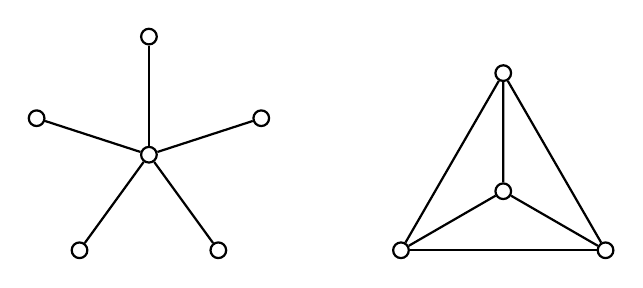
\begin{tikzpicture}
[nodedecorate/.style={shape=circle,inner sep=2pt,draw,thick},%
  linedecorate/.style={-,thick},%
  scale=1.5]
%%
%% complete bipartite graph K_{1,5}
%% nodes or vertices
\foreach \nodename/\x/\y in {1/0.9510/0.3090, 2/0/1, 3/-0.9510/0.3090,
  4/-0.5877/-0.8090, 5/0.5877/-0.8090, 6/0/0} {
  \node (\nodename) at (\x,\y) [nodedecorate] {};
}
%% edges or lines
\path
\foreach \startnode/\endnode in {1/6, 2/6, 3/6, 4/6, 5/6} {
  (\startnode) edge[linedecorate] node {} (\endnode)
};
%%
%% wheel graph W_4
%% nodes or vertices
\foreach \nodename/\x/\y in {1/3.866/-0.809, 2/3/0.691, 3/2.134/-0.809,
  4/3/-0.309} {
  \node (\nodename) at (\x,\y) [nodedecorate] {};
}
%% edges or lines
\path
\foreach \startnode/\endnode in {1/2, 1/3, 1/4, 2/3, 2/4, 3/4} {
  (\startnode) edge[linedecorate] node {} (\endnode)
};
\end{tikzpicture}
\caption{The vertex disjoint union $K_{1,5} \cup W_4$.}
\label{fig:introduction:vertex_disjoint_union_K15_W4}
\end{figure}

\begin{figure}[!htbp]
\centering
%%
%% graph G_1
\subfigure[$G_1$]{
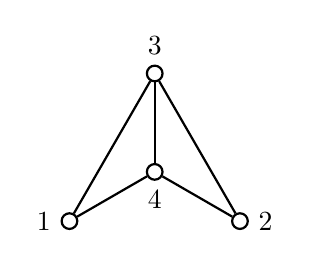
\begin{tikzpicture}
[nodedecorate/.style={shape=circle,inner sep=2pt,draw,thick},%
  linedecorate/.style={-,thick},%
  scale=1.25]
%% nodes or vertices
\foreach \nodename/\x/\y/\direction/\navigate in {
  1/-0.8660/-0.5/left/west, 2/0.8660/-0.5/right/east,
  3/0/1/above/north, 4/0/0/below/south} {
  \node (\nodename) at (\x,\y) [nodedecorate] {};
  \node [\direction] at (\nodename.\navigate) {$\nodename$};
}
%% edges or lines
\path
\foreach \startnode/\endnode in {1/3, 1/4, 2/3, 2/4, 3/4} {
  (\startnode) edge[linedecorate] node {} (\endnode)
};
\end{tikzpicture}
}
%%
%% graph G_2
\subfigure[$G_2$]{
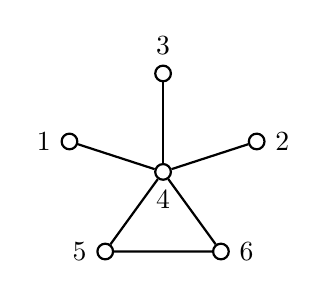
\begin{tikzpicture}
[nodedecorate/.style={shape=circle,inner sep=2pt,draw,thick},%
  linedecorate/.style={-,thick},%
  scale=1.25]
%% nodes or vertices
\foreach \nodename/\x/\y/\direction/\navigate in {
  1/-0.9510/0.3090/left/west, 2/0.9510/0.3090/right/east,
  3/0/1/above/north, 4/0/0/below/south, 5/-0.5877/-0.8090/left/west,
  6/0.5877/-0.8090/right/east} {
  \node (\nodename) at (\x,\y) [nodedecorate] {};
  \node [\direction] at (\nodename.\navigate) {$\nodename$};
}
%% edges or lines
\path
\foreach \startnode/\endnode in {1/4, 2/4, 3/4, 4/5, 4/6, 5/6} {
  (\startnode) edge[linedecorate] node {} (\endnode)
};
\end{tikzpicture}
}
%%
%% graph G_1 union G_2
\subfigure[$G_1 \cup G_2$]{
\label{fig:introduction:union_graphs_overlapping_vertex_sets}
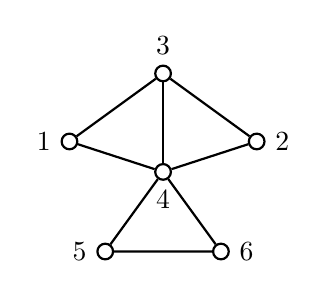
\begin{tikzpicture}
[nodedecorate/.style={shape=circle,inner sep=2pt,draw,thick},%
  linedecorate/.style={-,thick},%
  scale=1.25]
%% nodes or vertices
\foreach \nodename/\x/\y/\direction/\navigate in {
  1/-0.9510/0.3090/left/west, 2/0.9510/0.3090/right/east,
  3/0/1/above/north, 4/0/0/below/south, 5/-0.5877/-0.8090/left/west,
  6/0.5877/-0.8090/right/east} {
  \node (\nodename) at (\x,\y) [nodedecorate] {};
  \node [\direction] at (\nodename.\navigate) {$\nodename$};
}
%% edges or lines
\path
\foreach \startnode/\endnode in {1/4, 1/3, 2/3, 2/4, 3/4, 4/5, 4/6, 5/6} {
  (\startnode) edge[linedecorate] node {} (\endnode)
};
\end{tikzpicture}
}
%%
%% graph G_1 intersect G_2
\subfigure[$G_1 \cap G_2$]{
\label{fig:introduction:intersection_graphs_overlapping_vertex_sets}
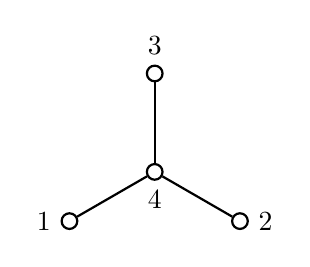
\begin{tikzpicture}
[nodedecorate/.style={shape=circle,inner sep=2pt,draw,thick},%
  linedecorate/.style={-,thick},%
  scale=1.25]
%% nodes or vertices
\foreach \nodename/\x/\y/\direction/\navigate in {
  1/-0.8660/-0.5/left/west, 2/0.8660/-0.5/right/east,
  3/0/1/above/north, 4/0/0/below/south} {
  \node (\nodename) at (\x,\y) [nodedecorate] {};
  \node [\direction] at (\nodename.\navigate) {$\nodename$};
}
%% edges or lines
\path
\foreach \startnode/\endnode in {1/4, 2/4, 3/4} {
  (\startnode) edge[linedecorate] node {} (\endnode)
};
\end{tikzpicture}
}
\caption{The union and intersection of graphs with overlapping vertex sets.}
\label{fig:introduction:union_intersection_graphs_overlapping_vertex_sets}
\end{figure}

The \emph{intersection} of graphs is defined as follows. For two
graphs $G_1 = (V_1, E_1)$ and $G_2 = (V_2, E_2)$, their intersection
is the graph
\[
G_1 \cap G_2
=
(V_1 \cap V_2,\, E_1 \cap E_2).
\]
Figure~\ref{fig:introduction:intersection_graphs_overlapping_vertex_sets}
illustrates the intersection of two graphs whose vertex sets overlap.
\index{graph!intersection}

The \emph{symmetric difference} of graphs is defined as follows. For
two graphs $G_1 = (V_1, E_1)$ and $G_2 = (V_2, E_2)$, their symmetric
difference is the graph
\[
G_1 \Delta G_2
=
(V, E)
\]
where $V = V_1 \Delta V_2$ and the edge set is given by
\[
E
=
(E_1 \Delta E_2) \backslash
\{
uv \;|\; u \in V_1 \cap V_2 \quad\text{or}\quad v \in V_1 \cap V_2
\}.
\]
Recall that the symmetric difference of two sets $S_1$ and $S_2$ is
defined by
\[
S_1 \Delta S_2
=
\{x \in S_1 \cup S_2 \;|\; x \notin S_1 \cap S_2\}.
\]
In the case where $V_1 = V_2$, then $G_1 \Delta G_2$ is simply the
empty graph. See Figure~\ref{fig:introduction:symmetric_difference}
for an illustration of the symmetric difference of two graphs.
\index{$\Delta$}
\index{symmetric difference}
\index{graph!symmetric difference}

\begin{figure}[!htbp]
\centering
%%
%% graph G_1
\subfigure[$G_1$]{
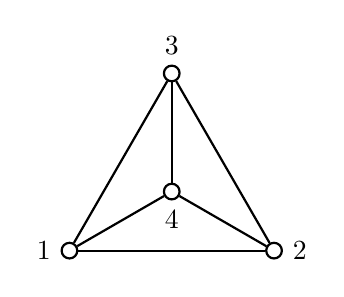
\begin{tikzpicture}
[nodedecorate/.style={shape=circle,inner sep=2pt,draw,thick},%
  linedecorate/.style={-,thick},%
  scale=1.5]
%% nodes or vertices
\foreach \nodename/\x/\y/\direction/\navigate in {
  1/-0.8660/-0.5/left/west, 2/0.8660/-0.5/right/east,
  3/0/1/above/north, 4/0/0/below/south} {
  \node (\nodename) at (\x,\y) [nodedecorate] {};
  \node [\direction] at (\nodename.\navigate) [] {$\nodename$};
}
%% edges or lines
\path
\foreach \startnode/\endnode in {1/2, 1/3, 1/4, 2/3, 2/4, 3/4} {
  (\startnode) edge[linedecorate] node {} (\endnode)
};
\end{tikzpicture}
}
\quad
%%
%% graph G_2
\subfigure[$G_2$]{
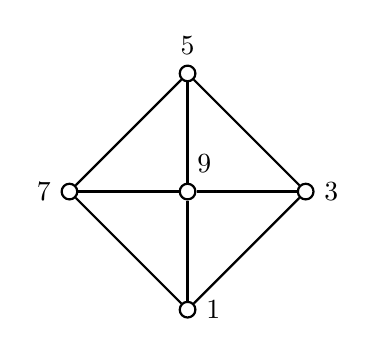
\begin{tikzpicture}
[nodedecorate/.style={shape=circle,inner sep=2pt,draw,thick},%
  linedecorate/.style={-,thick},%
  scale=1.5]
%% nodes or vertices
\foreach \nodename/\x/\y/\direction/\navigate in {
  1/0/-1/right/east, 3/1/0/right/east, 5/0/1/above/north,
  7/-1/0/left/west, 9/0/0/above right/north} {
  \node (\nodename) at (\x,\y) [nodedecorate] {};
  \node [\direction] at (\nodename.\navigate) [] {$\nodename$};
}
%% edges or lines
\path
\foreach \startnode/\endnode in {1/3, 1/7, 1/9, 3/5, 3/9, 5/7, 5/9, 7/9} {
  (\startnode) edge[linedecorate] node {} (\endnode)
};
\end{tikzpicture}
}
\quad
%%
%% graph G_1 symmetric difference G_2
\subfigure[$G_1 \Delta G_2$]{
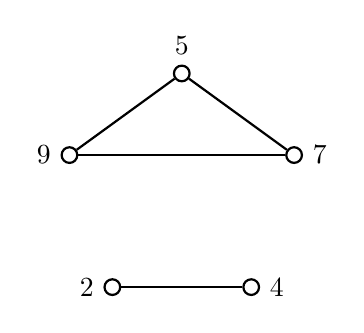
\begin{tikzpicture}
[nodedecorate/.style={shape=circle,inner sep=2pt,draw,thick},%
  linedecorate/.style={-,thick},%
  scale=1.5]
%% nodes or vertices
\foreach \nodename/\x/\y/\direction/\navigate in {
  2/-0.5877/-0.8090/left/west, 4/0.5877/-0.8090/right/east,
  5/0/1/above/north, 7/0.9510/0.3090/right/east,
  9/-0.9510/0.3090/left/west} {
  \node (\nodename) at (\x,\y) [nodedecorate] {};
  \node [\direction] at (\nodename.\navigate) {$\nodename$};
}
%% edges or lines
\path
\foreach \startnode/\endnode in {2/4, 5/7, 5/9, 7/9} {
  (\startnode) edge[linedecorate] node {} (\endnode)
};
\end{tikzpicture}
}
\caption{The symmetric difference of graphs.}
\label{fig:introduction:symmetric_difference}
\end{figure}

The \emph{join} of two disjoint graphs $G_1$ and $G_2$, denoted
$G_1 + G_2$, is their graph union, with each vertex of one graph
connecting to each vertex of the other graph. For example, the join of
the cycle graph $C_{n-1}$ with a single vertex graph is the
\emph{wheel graph} $W_n$. Figure~\ref{fig:introduction:wheel_graphs}
shows various wheel graphs.
\index{graph!join}
\index{wheel graph}

\begin{figure}[!htbp]
\centering
%%
%% wheel graph W_4
\subfigure[$W_4$]{
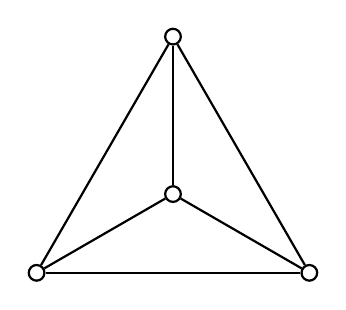
\begin{tikzpicture}
[nodedecorate/.style={shape=circle,inner sep=2pt,draw,thick},%
  linedecorate/.style={-,thick},%
  scale=2]
%% nodes or vertices
\foreach \nodename/\x/\y in {1/0.8660/-0.5, 2/0/1, 3/-0.8660/-0.5,
  4/0/0} {
  \node (\nodename) at (\x,\y) [nodedecorate] {};
}
%% edges or lines
\path
\foreach \startnode/\endnode in {1/2, 1/3, 1/4, 2/3, 2/4, 3/4} {
  (\startnode) edge[linedecorate] node {} (\endnode)
};
\end{tikzpicture}
}
\quad
%%
%% wheel graph W_5
\subfigure[$W_5$]{
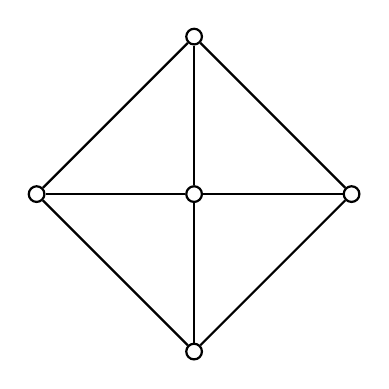
\begin{tikzpicture}
[nodedecorate/.style={shape=circle,inner sep=2pt,draw,thick},%
  linedecorate/.style={-,thick},%
  scale=2]
%% nodes or vertices
\foreach \nodename/\x/\y in {1/1/0, 2/0/1, 3/-1/0, 4/0/-1, 5/0/0} {
  \node (\nodename) at (\x,\y) [nodedecorate] {};
}
%% edges or lines
\path
\foreach \startnode/\endnode in {1/2, 1/4, 1/5, 2/3, 2/5, 3/4, 3/5,
  4/5} {
  (\startnode) edge[linedecorate] node {} (\endnode)
};
\end{tikzpicture}
}
\quad
%%
%% wheel graph W_6
\subfigure[$W_6$]{
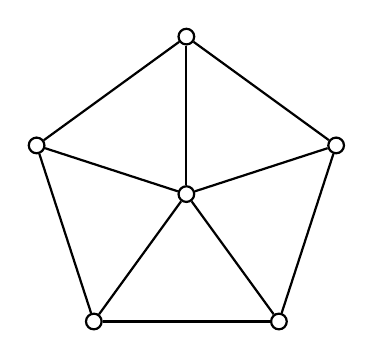
\begin{tikzpicture}
[nodedecorate/.style={shape=circle,inner sep=2pt,draw,thick},%
  linedecorate/.style={-,thick},%
  scale=2]
%% nodes or vertices
\foreach \nodename/\x/\y in {1/0.9510/0.3090, 2/0/1, 3/-0.9510/0.3090,
  4/-0.5877/-0.8090, 5/0.5877/-0.8090, 6/0/0} {
  \node (\nodename) at (\x,\y) [nodedecorate] {};
}
%% edges or lines
\path
\foreach \startnode/\endnode in {1/2, 1/5, 1/6, 2/3, 2/6, 3/4, 3/6,
  4/5, 4/6, 5/6} {
  (\startnode) edge[linedecorate] node {} (\endnode)
};
\end{tikzpicture}
}
%%
%% wheel graph W_7
\subfigure[$W_7$]{
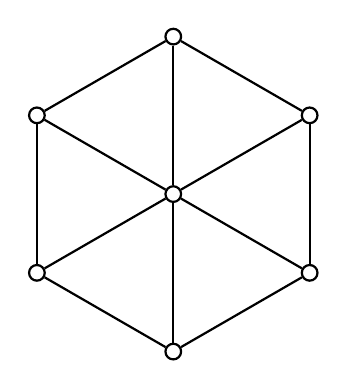
\begin{tikzpicture}
[nodedecorate/.style={shape=circle,inner sep=2pt,draw,thick},%
  linedecorate/.style={-,thick},%
  scale=2]
%% nodes or vertices
\foreach \nodename/\x/\y in {1/0.8660/0.5, 2/0/1, 3/-0.8660/0.5,
  4/-0.8660/-0.5, 5/0/-1, 6/0.8660/-0.5, 7/0/0} {
  \node (\nodename) at (\x,\y) [nodedecorate] {};
}
%% edges or lines
\path
\foreach \startnode/\endnode in {1/2, 1/6, 1/7, 2/3, 2/7, 3/4, 3/7,
  4/5, 4/7, 5/6, 5/7, 6/7} {
  (\startnode) edge[linedecorate] node {} (\endnode)
};
\end{tikzpicture}
}
\quad
%%
%% wheel graph W_8
\subfigure[$W_8$]{
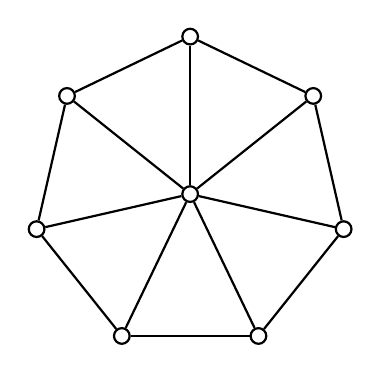
\begin{tikzpicture}
[nodedecorate/.style={shape=circle,inner sep=2pt,draw,thick},%
  linedecorate/.style={-,thick},%
  scale=2]
%% nodes or vertices
\foreach \nodename/\x/\y in {1/0.7818/0.6234, 2/0/1, 3/-0.7818/0.6234,
  4/-0.9749/-0.2225, 5/-0.4338/-0.9009, 6/0.4338/-0.9009,
  7/0.9749/-0.2225, 8/0/0} {
  \node (\nodename) at (\x,\y) [nodedecorate] {};
}
%% edges or lines
\path
\foreach \startnode/\endnode in {1/2, 1/7, 1/8, 2/3, 2/8, 3/4, 3/8,
  4/5, 4/8, 5/6, 5/8, 6/7, 6/8, 7/8} {
  (\startnode) edge[linedecorate] node {} (\endnode)
};
\end{tikzpicture}
}
\quad
%%
%% wheel graph W_9
\subfigure[$W_9$]{
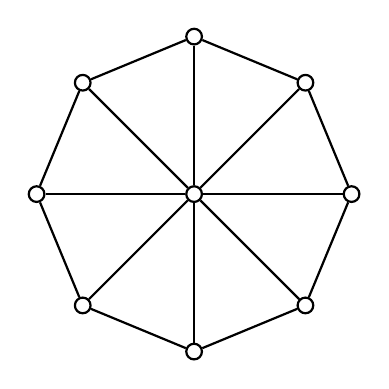
\begin{tikzpicture}
[nodedecorate/.style={shape=circle,inner sep=2pt,draw,thick},%
  linedecorate/.style={-,thick},%
  scale=2]
%% nodes or vertices
\foreach \nodename/\x/\y in {1/1/0, 2/0.7071/0.7071, 3/0/1,
  4/-0.7071/0.7071, 5/-1/0, 6/-0.7071/-0.7071, 7/0/-1,
  8/0.7071/-0.7071, 9/0/0} {
  \node (\nodename) at (\x,\y) [nodedecorate] {};
}
%% edges or lines
\path
\foreach \startnode/\endnode in {1/2, 1/8, 1/9, 2/3, 2/9, 3/4, 3/9,
  4/5, 4/9, 5/6, 5/9, 6/7, 6/9, 7/8, 7/9, 8/9} {
  (\startnode) edge[linedecorate] node {} (\endnode)
};
\end{tikzpicture}
}
\caption{The wheel graphs $W_n$ for $n = 4,\dots,9$.}
\label{fig:introduction:wheel_graphs}
\end{figure}


%%--- Edge or vertex deletion -------------------------------------------%%

\subsection{Edge or vertex deletion/insertion}


%%--- Vertex deletion subgraph ------------------------------------------%%

\subsubsection{Vertex deletion subgraph}

\index{vertex deletion subgraph}
If $G = (V,E)$ is any graph with at least $2$ vertices, then the
\emph{vertex deletion subgraph} is the subgraph obtained from $G$ by
deleting a vertex $v \in V$ and also all the edges incident to that
vertex. The vertex deletion subgraph of $G$ is sometimes denoted
$G - \{v\}$.
Sage can compute vertex deletions, as the following example shows.
%
\begin{center}
\fontsize{9pt}{9pt}
\selectfont
\tt
\begin{lstlisting}
sage: G = Graph({1: [2,4], 2: [1,4], 3: [2,6], 4: [1,3], 5: [4,2], 6: [3,1]})
sage: G.vertices()
[1, 2, 3, 4, 5, 6]
sage: E1 = Set(G.edges(labels=False)); E1
{(1, 2), (4, 5), (1, 4), (2, 3), (3, 6), (1, 6), (2, 5), (3, 4), (2, 4)}
sage: E4 = Set(G.edges_incident(vertices=[4], labels=False)); E4
{(4, 5), (3, 4), (2, 4), (1, 4)}
sage: G.delete_vertex(4)
sage: G.vertices()
[1, 2, 3, 5, 6]
sage: E2 = Set(G.edges(labels=False)); E2
{(1, 2), (1, 6), (2, 5), (2, 3), (3, 6)}
sage: E1.difference(E2) == E4
True
\end{lstlisting}
\end{center}
%
Figure~\ref{fig:introduction:vertex_deletion_subgraphs}
presents a sequence of subgraphs obtained by repeatedly deleting
vertices. As the figure shows, when a vertex is deleted from a graph,
all edges incident on that vertex are deleted as well.

\begin{figure}[!htbp]
\centering
%%
%% graph G
\subfigure[$G$]{
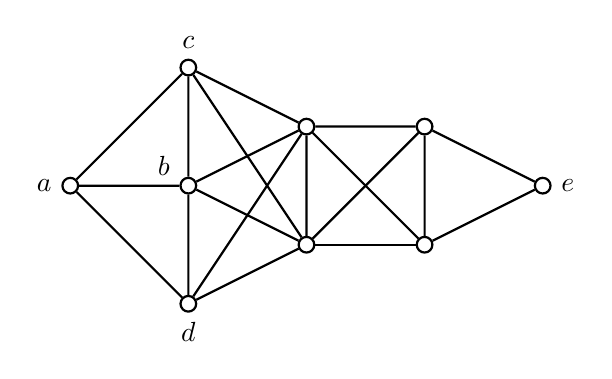
\begin{tikzpicture}
[nodedecorate/.style={shape=circle,inner sep=2pt,draw,thick},%
  linedecorate/.style={-,thick}, scale=1.5]
%% nodes or vertices
\foreach \nodename/\x/\y in {a/0/1, b/1/1, c/1/2, d/1/0, 1/2/1.5,
  2/2/0.5, 3/3/1.5, 4/3/0.5, e/4/1} {
  \node (\nodename) at (\x,\y) [nodedecorate] {};
}
\foreach \nodename/\direction/\navigate in {a/left/west,
  b/above left/west, c/above/north, d/below/south, e/right/east} {
  \node [\direction] at (\nodename.\navigate) {$\nodename$};
}
%% edges or lines
\path
\foreach \startnode/\endnode in {a/b, a/c, a/d, b/c, b/d, b/1, b/2,
  c/1, c/2, d/1, d/2, 1/2, 1/3, 1/4, 2/3, 2/4, 3/4, 3/e, 4/e} {
  (\startnode) edge[linedecorate] node {} (\endnode)
};
\end{tikzpicture}
}
%%
%% vertex deletion subgraph G - {b}
\subfigure[$G - \{b\}$]{
\begin{tikzpicture}
[nodedecorate/.style={shape=circle,inner sep=2pt,draw,thick},%
  linedecorate/.style={-,thick}, scale=1.5]
%% nodes or vertices
\foreach \nodename/\x/\y in {a/0/1, c/1/2, d/1/0, 1/2/1.5, 2/2/0.5,
  3/3/1.5, 4/3/0.5, e/4/1} {
  \node (\nodename) at (\x,\y) [nodedecorate] {};
}
\foreach \nodename/\direction/\navigate in {a/left/west,
  c/above/north, d/below/south, e/right/east} {
  \node [\direction] at (\nodename.\navigate) {$\nodename$};
}
%% edges or lines
\path
\foreach \startnode/\endnode in {a/c, a/d, c/1, c/2, d/1, d/2, 1/2,
  1/3, 1/4, 2/3, 2/4, 3/4, 3/e, 4/e} {
  (\startnode) edge[linedecorate] node {} (\endnode)
};
\end{tikzpicture}
}
%%
%% vertex deletion subgraph G - {a,b}
\subfigure[$G - \{a, b\}$]{
\begin{tikzpicture}
[nodedecorate/.style={shape=circle,inner sep=2pt,draw,thick},%
  linedecorate/.style={-,thick}, scale=1.5]
%% nodes or vertices
\foreach \nodename/\x/\y in {c/1/2, d/1/0, 1/2/1.5, 2/2/0.5, 3/3/1.5,
  4/3/0.5, e/4/1} {
  \node (\nodename) at (\x,\y) [nodedecorate] {};
}
\foreach \nodename/\direction/\navigate in {c/left/west,
  d/left/west, e/right/east} {
  \node [\direction] at (\nodename.\navigate) {$\nodename$};
}
%% edges or lines
\path
\foreach \startnode/\endnode in {c/1, c/2, d/1, d/2, 1/2, 1/3, 1/4,
  2/3, 2/4, 3/4, 3/e, 4/e} {
  (\startnode) edge[linedecorate] node {} (\endnode)
};
\end{tikzpicture}
}
%%
%% vertex deletion subgraph G - {a,b,e}
\subfigure[$G - \{a, b, e\}$]{
\begin{tikzpicture}
[nodedecorate/.style={shape=circle,inner sep=2pt,draw,thick},%
  linedecorate/.style={-,thick}, scale=1.5]
%% nodes or vertices
\foreach \nodename/\x/\y in {c/1/2, d/1/0, 1/2/1.5, 2/2/0.5, 3/3/1.5,
  4/3/0.5} {
  \node (\nodename) at (\x,\y) [nodedecorate] {};
}
\foreach \nodename/\direction/\navigate in {c/left/west,
  d/left/west} {
  \node [\direction] at (\nodename.\navigate) {$\nodename$};
}
%% edges or lines
\path
\foreach \startnode/\endnode in {c/1, c/2, d/1, d/2, 1/2, 1/3, 1/4,
  2/3, 2/4, 3/4} {
  (\startnode) edge[linedecorate] node {} (\endnode)
};
\end{tikzpicture}
}
%%
%% vertex deletion subgraph G - {a,b,c,d,e}
\subfigure[$G - \{a, b, c, d, e\}$]{
\begin{tikzpicture}
[nodedecorate/.style={shape=circle,inner sep=2pt,draw,thick},%
  linedecorate/.style={-,thick}, scale=1.5]
%% nodes or vertices
\foreach \nodename/\x/\y in {1/2/1.5, 2/2/0.5, 3/3/1.5, 4/3/0.5} {
  \node (\nodename) at (\x,\y) [nodedecorate] {};
}
%% a stub node that should not be visible
\node (stubLeft) at (0,1.5) [] {};
\node (stubRight) at (5,1.5) [] {};
%% edges or lines
\path
\foreach \startnode/\endnode in {1/2, 1/3, 1/4, 2/3, 2/4, 3/4} {
  (\startnode) edge[linedecorate] node {} (\endnode)
};
\end{tikzpicture}
}
\caption{Obtaining subgraphs via repeated vertex deletion.}
\label{fig:introduction:vertex_deletion_subgraphs}
\end{figure}


%%--- Edge deletion subgraph --------------------------------------------%%

\subsubsection{Edge deletion subgraph}

\index{edge deletion subgraph}
If $G = (V,E)$ is any graph with at least $1$ edge, then the
\emph{edge deletion subgraph} is the subgraph obtained from $G$ by
deleting an edge $e \in E$, but not the vertices incident to that edge.
The edge deletion subgraph of $G$ is sometimes denoted $G - \{e\}$.
Sage can compute edge deletions, as the following example shows.
%
\begin{center}
\fontsize{9pt}{9pt}
\selectfont
\tt
\begin{lstlisting}
sage: G = Graph({1: [2,4], 2: [1,4], 3: [2,6], 4: [1,3], 5: [4,2], 6: [3,1]})
sage: E1 = Set(G.edges(labels=False)); E1
{(1, 2), (4, 5), (1, 4), (2, 3), (3, 6), (1, 6), (2, 5), (3, 4), (2, 4)}
sage: V1 = G.vertices(); V1
[1, 2, 3, 4, 5, 6]
sage: E14 = Set([(1,4)]); E14
{(1, 4)}
sage: G.delete_edge([1,4])
sage: E2 = Set(G.edges(labels=False)); E2
{(1, 2), (4, 5), (2, 3), (3, 6), (1, 6), (2, 5), (3, 4), (2, 4)}
sage: E1.difference(E2) == E14
True
\end{lstlisting}
\end{center}
%
Figure~\ref{fig:introduction:edge_deletion_subgraphs} shows a sequence
of graphs resulting from edge deletion. Unlike vertex deletion, when
an edge is deleted the vertices incident on that edge are left
intact.

\begin{figure}[!htbp]
\centering
%%
%% graph G
\subfigure[$G$]{
\begin{tikzpicture}
[nodedecorate/.style={shape=circle,inner sep=2pt,draw,thick},%
  linedecorate/.style={-,thick}, scale=1.6]
%% nodes or vertices
\foreach \nodename/\x/\y in {a/0.8660/-0.5, b/0/1, c/-0.8660/-0.5,
  d/0/0} {
  \node (\nodename) at (\x,\y) [nodedecorate] {};
}
\foreach \nodename/\direction/\navigate in {a/right/east, b/above/north,
  c/left/west} {
  \node [\direction] at (\nodename.\navigate) {$\nodename$};
}
%% edges or lines
\path
\foreach \startnode/\endnode in {a/b, a/c, a/d, b/c, b/d, c/d} {
  (\startnode) edge[linedecorate] node {} (\endnode)
};
\end{tikzpicture}
}
%%
%% edge deletion subgraph G - {ac}
\subfigure[$G - \{ac\}$]{
\begin{tikzpicture}
[nodedecorate/.style={shape=circle,inner sep=2pt,draw,thick},%
  linedecorate/.style={-,thick}, scale=1.6]
%% nodes or vertices
\foreach \nodename/\x/\y in {a/0.8660/-0.5, b/0/1, c/-0.8660/-0.5,
  d/0/0} {
  \node (\nodename) at (\x,\y) [nodedecorate] {};
}
\foreach \nodename/\direction/\navigate in {a/right/east, b/above/north,
  c/left/west} {
  \node [\direction] at (\nodename.\navigate) {$\nodename$};
}
%% edges or lines
\path
\foreach \startnode/\endnode in {a/b, a/d, b/c, b/d, c/d} {
  (\startnode) edge[linedecorate] node {} (\endnode)
};
\end{tikzpicture}
}
%%
%% edge deletion subgraph G - {ab, ac, bc}
\subfigure[$G - \{ab, ac, bc\}$]{
\label{fig:introduction:skeleton_subgraph_via_edge_deletion}
\begin{tikzpicture}
[nodedecorate/.style={shape=circle,inner sep=2pt,draw,thick},%
  linedecorate/.style={-,thick}, scale=1.6]
%% nodes or vertices
\foreach \nodename/\x/\y in {a/0.8660/-0.5, b/0/1, c/-0.8660/-0.5,
  d/0/0} {
  \node (\nodename) at (\x,\y) [nodedecorate] {};
}
\foreach \nodename/\direction/\navigate in {a/right/east, b/above/north,
  c/left/west} {
  \node [\direction] at (\nodename.\navigate) {$\nodename$};
}
%% edges or lines
\path
\foreach \startnode/\endnode in {a/d, b/d, c/d} {
  (\startnode) edge[linedecorate] node {} (\endnode)
};
\end{tikzpicture}
}
\caption{Obtaining subgraphs via repeated edge deletion.}
\label{fig:introduction:edge_deletion_subgraphs}
\end{figure}


%%--- Vertex cut, cut vertex, or cutpoint -------------------------------%%

\subsubsection{Vertex cut, cut vertex, or cutpoint}
\index{graph!cut}
\index{separating set}
\index{vertex cut}

A \emph{vertex cut} (or \emph{separating set}) of a connected graph
$G = (V, E)$ is a subset $W \subseteq V$ such that the vertex deletion
subgraph $G - W$ is disconnected. In fact, if $v_1, v_2 \in V$ are two
non-adjacent vertices, then you can ask for a vertex cut $W$ for which
$v_1, v_2$ belong to different components of $G - W$. Sage's
\verb!vertex_cut! method allows you to compute a minimal cut having
this property. For many connected graphs, the removal of a single
vertex is sufficient for the graph to be disconnected
(see Figure~\ref{fig:introduction:skeleton_subgraph_via_edge_deletion}).
%% What about the case where a graph is already disconnected? How would
%% you define a vertex cut in a disconnected graph? That would involve
%% defining "graph components", so that a vertex cut is a single vertex
%% or a set of vertices that would result in more components.


%%--- Edge cut, cut edge, or bridge -------------------------------------%%

\subsubsection{Edge cut, cut edge, or bridge}
\index{bond}
\index{bridge}
\index{cut set}
\index{disconnecting set}
\index{edge cut}

If deleting a single, specific edge would disconnect a graph $G$, that
edge is called a \emph{bridge}. More generally, the \emph{edge cut}
(or \emph{disconnecting set} or \emph{seg}) of a connected graph
$G = (V, E)$ is a set of edges $F \subseteq E$ whose removal yields an
edge deletion subgraph $G - F$ that is disconnected. A minimal edge
cut is called a \emph{cut set} or a \emph{bond}.
In fact, if $v_1, v_2 \in V$ are two vertices, then you can ask for an
edge cut $F$ for which $v_1, v_2$ belong to different components of
$G - F$. Sage's \verb!edge_cut! method allows you to compute a minimal
cut having this property. For example, any of the three edges in
Figure~\ref{fig:introduction:skeleton_subgraph_via_edge_deletion}
qualifies as a bridge and those three edges form an edge cut for the
graph in question.

\begin{theorem}
Let $G$ be a connected graph. An edge $e \in E(G)$ is a bridge of $G$
if and only if $e$ does not lie on a cycle of $G$.
\end{theorem}

\begin{proof}
First, assume that $e = uv$ is a bridge of $G$. Suppose for
contradiction that $e$ lies on a cycle
\[
C: u, v, w_1, w_2, \dots, w_k, u.
\]
Then $G - e$ contains a $u$-$v$ path
$u, w_k, \dots, w_2, w_1, v$. Let $u_1, v_1$ be any two vertices in
$G - e$. By hypothesis, $G$ is connected so there is a $u_1$-$v_1$
path $P$ in $G$. If $e$ does not lie on $P$, then $P$ is also a path
in $G - e$ so that $u_1, v_1$ are connected, which contradicts our
assumption of $e$ being a bridge. On the other hand, if $e$ lies on
$P$, then express $P$ as
\[
u_1, \dots, u, v, \dots, v_1
\quad\text{or}\quad
u_1, \dots, v, u, \dots, v_1.
\]
Now
\[
u_1, \dots, u, w_k, \dots, w_2, w_1, v, \dots, v_1
\quad\text{or}\quad
u_1, \dots, v, w_1, w_2, \dots, w_k, u, \dots, v_1
\]
respectively is a $u_1$-$v_1$ walk in $G - e$. By
Theorem~\ref{thm:introduction:every_walk_has_a_path}, $G - e$
contains a $u_1$-$v_1$ path, which contradicts our assumption about
$e$ being a bridge.

Conversely, let $e = uv$ be an edge that does not lie on any cycles of
$G$. If $G - e$ has no $u$-$v$ paths, then we are done. Otherwise,
assume for contradiction that $G - e$ has a $u$-$v$ path $P$. Then $P$
with $uv$ produces a cycle in $G$. This cycle contains $e$, in
contradiction of our assumption that $e$ does not lie on any cycles of
$G$.
\end{proof}


%%--- Edge contraction --------------------------------------------------%%

\subsubsection{Edge contraction}

An \emph{edge contraction} is an operation which, like edge deletion,
removes an edge from a graph. However, unlike edge deletion, edge
contraction also merges together the two vertices the edge used to
connect. For a graph $G = (V, E)$ and an edge $uv = e \in E$, the edge
contraction $G/e$ is the graph obtained as follows:
%
\begin{enumerate}
\item Delete the vertices $u,v$ from $G$.

\item In place of $u,v$ is a new vertex $v_e$.

\item The vertex $v_e$ is adjacent to vertices that were adjacent
  to $u$, $v$, or both $u$ and $v$.
\end{enumerate}
\index{edge contraction}
The vertex set of $G/e = (V', E')$ is defined as
$V' = \big(V \backslash \{u,v\}\big) \cup \{v_e\}$ and its edge set is
\[
E'
=
\big\{
wx \in E \;\left.\right|\; \{w,x\} \cap \{u,v\} = \emptyset
\big\}
\cup
\big\{
v_e w
\;\left.\right|\;
uw \in E \backslash \{e\} \;\text{or}\; vw \in E \backslash \{e\}
\big\}.
\]
Make the substitutions
%
\begin{align*}
E_1 &= \big\{
wx \in E \;\left.\right|\; \{w,x\} \cap \{u,v\} = \emptyset \big\} \\
E_2 &= \big\{
v_e w \;\left.\right|\;
uw \in E \backslash \{e\} \;\text{or}\; vw \in E \backslash \{e\} \big\}.
\end{align*}
%
Let $G$ be the wheel graph $W_6$ in
Figure~\ref{fig:introduction:contracting_wheel_graph_W6} and consider
the edge contraction $G/ab$, where $ab$ is the gray colored edge in
that figure. Then the edge set $E_1$ denotes all those edges in $G$
each of which is not incident on $a$, $b$, or both $a$ and $b$. These
are precisely those edges that are colored red. The edge set $E_2$
means that we consider those edges in $G$ each of which is incident on
exactly one of $a$ or $b$, but not both. The blue colored edges in
Figure~\ref{fig:introduction:contracting_wheel_graph_W6} are precisely
those edges that $E_2$ suggests for consideration. The result of the
edge contraction $G/ab$ is the wheel graph $W_5$ in
Figure~\ref{fig:introduction:contracting_wheel_graph_W5}.
Figures~\ref{fig:introduction:contracting_wheel_graph_W6}
to~\ref{fig:introduction:wheel_graph_W6_contracted_to_K1} present a
sequence of edge contractions that starts with $W_6$ and repeatedly
contracts it to the trivial graph $K_1$.

\begin{figure}[!htbp]
\centering
%%
%% wheel graph W_6
\subfigure[$G_1$]{
\label{fig:introduction:contracting_wheel_graph_W6}
\begin{tikzpicture}
[nodedecorate/.style={shape=circle,inner sep=2pt,draw,thick},%
  linedecorate/.style={-,very thick},%
  scale=1.7]
%% nodes or vertices
\foreach \nodename/\x/\y/\direction/\navigate in {
  a/-0.5877/-0.8090/left/west, b/0.5877/-0.8090/right/east,
  c/0.9510/0.3090/right/east, d/0/1/above/north,
  e/-0.9510/0.3090/left/west, f/0/0/above right/north} {
  \node (\nodename) at (\x,\y) [nodedecorate] {};
  \node [\direction] at (\nodename.\navigate) {$\nodename$};
}
%% edges or lines
\path
\foreach \startnode/\endnode/\color in {c/d/red, c/b/blue, c/f/red,
  d/e/red, d/f/red, e/a/blue, e/f/red, a/b/gray, a/f/blue, b/f/blue} {
  (\startnode) edge[linedecorate,color=\color] node {} (\endnode)
};
\end{tikzpicture}
}
%%
%% edge contraction W_6/ab
\subfigure[$G_2 = G_1/ab$]{
\label{fig:introduction:contracting_wheel_graph_W5}
\begin{tikzpicture}
[nodedecorate/.style={shape=circle,inner sep=2pt,draw,thick},%
  linedecorate/.style={-,thick},%
  scale=1.7]
%% nodes or vertices
\foreach \nodename/\x/\y/\direction/\navigate in {c/1/0/right/east,
  d/0/1/above/north, e/-1/0/left/west, f/0/0/above right/north} {
  \node (\nodename) at (\x,\y) [nodedecorate] {};
  \node [\direction] at (\nodename.\navigate) {$\nodename$};
}
\node (ab) at (0,-1) [nodedecorate] {};
\node [right] at (ab.east) {$v_{ab} = g$};
%% edges or lines
\path
\foreach \startnode/\endnode in {c/d, c/ab, c/f, d/e, d/f, e/ab, e/f,
  ab/f} {
  (\startnode) edge[linedecorate] node {} (\endnode)
};
\end{tikzpicture}
}
%%
%% edge contraction G_2/cg
\subfigure[$G_3 = G_2/cg$]{
\begin{tikzpicture}
[nodedecorate/.style={shape=circle,inner sep=2pt,draw,thick},%
  linedecorate/.style={-,thick},%
  scale=1.7]
%% nodes or vertices
\foreach \nodename/\x/\y/\direction/\navigate in {d/0/1/above/north,
  e/-0.8660/-0.5/left/west, f/0/0/above right/north} {
  \node (\nodename) at (\x,\y) [nodedecorate] {};
  \node [\direction] at (\nodename.\navigate) {$\nodename$};
}
\node (cg) at (0.8660,-0.5) [nodedecorate] {};
\node [right] at (cg.east) {$v_{cg} = h$};
%% edges or lines
\path
\foreach \startnode/\endnode in {cg/d, cg/e, cg/f, d/e, d/f, e/f} {
  (\startnode) edge[linedecorate] node {} (\endnode)
};
\end{tikzpicture}
}
%%
%% edge contraction G_3/dh
\subfigure[$G_4 = G_3/dh$]{
\begin{tikzpicture}
[nodedecorate/.style={shape=circle,inner sep=2pt,draw,thick},%
  linedecorate/.style={-,thick},%
  scale=1.7]
%% nodes or vertices
\foreach \nodename/\x/\y/\direction/\navigate in {f/0/1/above/north,
  e/-0.8660/-0.5/left/west} {
  \node (\nodename) at (\x,\y) [nodedecorate] {};
  \node [\direction] at (\nodename.\navigate) {$\nodename$};
}
\node (dh) at (0.8660,-0.5) [nodedecorate] {};
\node [right] at (dh.east) {$v_{dh} = i$};
%% edges or lines
\path
\foreach \startnode/\endnode in {dh/f, dh/e, e/f} {
  (\startnode) edge[linedecorate] node {} (\endnode)
};
\end{tikzpicture}
}
%%
%% edge contraction G_4/fi
\subfigure[$G_5 = G_4/fi$]{
\begin{tikzpicture}
[nodedecorate/.style={shape=circle,inner sep=2pt,draw,thick},%
  linedecorate/.style={-,thick},%
  scale=1.7]
%% nodes or vertices
\node (e) at (-0.8660,-0.5) [nodedecorate] {};
\node [left] at (e.west) {$e$};
\node (fi) at (0.8660,-0.5) [nodedecorate] {};
\node [right] at (fi.east) {$v_{fi} = j$};
%% edges or lines
\path (e) edge[linedecorate] node {} (fi);
\end{tikzpicture}
}
%%
%% edge contraction G_5/ej
\subfigure[$G_6 = G_5/ej$]{
\label{fig:introduction:wheel_graph_W6_contracted_to_K1}
\begin{tikzpicture}
[nodedecorate/.style={shape=circle,inner sep=2pt,draw,thick},%
  linedecorate/.style={-,thick},%
  scale=1.7]
%% nodes or vertices
\node (ej) at (0,0) [nodedecorate] {};
\node [right] at (ej.east) {$v_{ej}$};
%% stub node that should not be visible
\node (stub1) at (1,0) [] {};
\node (stub2) at (-1,0) [] {};
\end{tikzpicture}
}
\caption{Contracting the wheel graph $W_6$ to the trivial graph $K_1$.}
\label{fig:introduction:edge_contraction_W6_to_K1}
\end{figure}


%%--- Complements -------------------------------------------------------%%

\subsection{Complements}

\index{$G^c$}
\index{complement}
\index{self-complementary graph}
\index{relative complement}
The \emph{complement} of a simple graph has the same vertices, but
exactly those edges that are not in the original graph. In other
words, if $G^c = (V, E^c)$ is the complement of $G = (V,E)$, then two
distinct vertices $v,w \in V$ are adjacent in $G^c$ if and only if
they are not adjacent in $G$. The sum of the adjacency matrix of $G$
and that of $G^c$ is the matrix with $1$'s everywhere, except for
$0$'s on the main diagonal. A simple graph that is isomorphic to its
complement is called a \emph{self-complementary graph}. Let $H$ be a
subgraph of $G$. The \emph{relative complement} of $G$ and $H$ is the
edge deletion subgraph $G - E(H)$. That is, we delete from $G$ all
edges in $H$. Sage can compute edge complements, as the following
example shows.
%
\begin{center}
\fontsize{9pt}{9pt}
\selectfont
\tt
\begin{lstlisting}
sage: G = Graph({1: [2,4], 2: [1,4], 3: [2,6], 4: [1,3], 5: [4,2], 6: [3,1]})
sage: Gc = G.complement()
sage: EG = Set(G.edges(labels=False)); EG
{(1, 2), (4, 5), (1, 4), (2, 3), (3, 6), (1, 6), (2, 5), (3, 4), (2, 4)}
sage: EGc = Set(Gc.edges(labels=False)); EGc
{(1, 5), (2, 6), (4, 6), (1, 3), (5, 6), (3, 5)}
sage: EG.difference(EGc) == EG
True
sage: EGc.difference(EG) == EGc
True
sage: EG.intersection(EGc)
{}
\end{lstlisting}
\end{center}

\begin{theorem}
If $G = (V, E)$ is self-complementary, then the order of $G$ is
$|V| = 4k$ or $|V| = 4k + 1$ for some non-negative integer
$k$. Furthermore, if $n = |V|$ is the order of $G$, then the size of
$G$ is $|E| = n(n - 1) / 4$.
\end{theorem}

\begin{proof}
Let $G$ be a self-complementary graph of order $n$. Each of $G$ and
$G^c$ contains half the number of edges in
$K_n$. From~(\ref{eq:introduction:size_of_K_n}), we have
\[
|E(G)|
=
|E(G^c)|
=
\frac{1}{2} \cdot \frac{n(n - 1)}{2}
=
\frac{n(n - 1)}{4}.
\]
Then $n \;|\; n(n - 1)$, with one of $n$ and $n - 1$ being even and
the other odd. If $n$ is even, $n - 1$ is odd so $\gcd(4, n-1) = 1$,
hence by~\cite[Theorem~1.9]{Shoup2008} we have $4 \;|\; n$ and so
$n = 4k$ for some non-negative $k \in \ZZ$. If $n - 1$ is even, use a
similar argument to conclude that $n = 4k + 1$ for some non-negative
$k \in \ZZ$.
\end{proof}


%%--- Cartesian product -------------------------------------------------%%

\subsection{Cartesian product}
\index{$\square$}
\index{Cartesian product}

The \emph{Cartesian product} $G \square H$ of graphs $G$ and $H$ is a
graph such that the vertex set of $G \square H$ is the Cartesian
product $V(G) \times V(H)$. Any two vertices $(u, u')$ and $(v, v')$
are adjacent in $G \square H$ if and only if either
%
\begin{enumerate}
\item $u = v$ and $u'$ is adjacent with $v'$ in $H$; or

\item $u' = v'$ and $u$ is adjacent with $v$ in $G$.
\end{enumerate}
The vertex set of $G \square H$ is $V(G \square H) = V(G) \times V(H)$
and the edge set of $G \square H$ is the union
\[
E(G \square H)
=
\big(V(G) \times E(H)\big) \cup \big(E(G) \times V(H)\big).
\]
%
Sage can compute Cartesian products, as the following example shows.
%
\begin{center}
\fontsize{9pt}{9pt}
\selectfont
\tt
\begin{lstlisting}
sage: Z = graphs.CompleteGraph(2); len(Z.vertices()); len(Z.edges())
2
1
sage: C = graphs.CycleGraph(5); len(C.vertices()); len(C.edges())
5
5
sage: P = C.cartesian_product(Z); len(P.vertices()); len(P.edges())
10
15
\end{lstlisting}
\end{center}

The \emph{path graph} $P_n$ is a tree with $n$ vertices
$V = \{v_1, v_2, \dots, v_n\}$ and edges
$E = \{ (v_i, v_{i+1}) \;|\; 1 \leq i \leq n-1 \}$. In this case,
$\deg(v_1) = \deg(v_n) = 1$ and $\deg(v_i) = 2$ for $1 < i < n$. The
path graph $P_n$ can be obtained from the cycle graph $C_n$ by
deleting one edge of $C_n$. The \emph{ladder graph} $L_n$ is the
Cartesian product of path graphs, i.e. $L_n = P_n \square P_1$.
\index{$L_n$}
\index{graph!ladder}
\index{graph!path}
\index{ladder graph}
\index{path graph}

The Cartesian product of two graphs $G_1$ and $G_2$ can be visualized
as follows. Let $V_1 = \{u_1, u_2, \dots, u_m\}$ and
$V_2 = \{v_1, v_2, \dots, v_n\}$ be the vertex sets of $G_1$ and
$G_2$, respectively. Let $H_1, H_2, \dots, H_n$ be $n$ copies of
$G_1$. Place each $H_i$ at the location of $v_i$ in $G_2$. Then
$u_i \in V(H_j)$ is adjacent to $u_i \in V(H_k)$ if and only if
$v_{jk} \in E(G_2)$. See
Figure~\ref{fig:introduction:Cartesian_product_K3_P3} for an
illustration of obtaining the Cartesian product of $K_3$ and $P_3$.

\begin{figure}[!htbp]
\centering
%%
%% graph K_3
\subfigure[$K_3$]{
\begin{tikzpicture}
[nodedecorate/.style={shape=circle,inner sep=2pt,draw,thick},%
  linedecorate/.style={-,thick},%
  scale=1]
%% nodes or vertices
\foreach \nodename/\x/\y in {1/0.8660/-0.5, 2/0/1, 3/-0.8660/-0.5} {
  \node (\nodename) at (\x,\y) [nodedecorate] {};
}
%% edges or lines
\path
\foreach \startnode/\endnode in {1/2, 1/3, 2/3} {
  (\startnode) edge[linedecorate] node {} (\endnode)
};
\end{tikzpicture}
}
\qquad
%%
%% graph P_3
\subfigure[$P_3$]{
\begin{tikzpicture}
[nodedecorate/.style={shape=circle,inner sep=2pt,draw,thick},%
  linedecorate/.style={-,thick}]
%% nodes or vertices
\foreach \nodename/\x/\y in {1/0/0, 2/0/1, 3/0/2} {
  \node (\nodename) at (\x,\y) [nodedecorate] {};
}
%% stub nodes that should not be visible
\node () at (-0.5,0) [] {};
\node () at (0.5,0) [] {};
%% edges or lines
\path
\foreach \startnode/\endnode in {1/2, 2/3} {
  (\startnode) edge[linedecorate] node {} (\endnode)
};
\end{tikzpicture}
}
\qquad
%%
%% K_3 Cartesian product P_3
\subfigure[$K_3 \square P_3$]{
\begin{tikzpicture}
[nodedecorate/.style={shape=circle,inner sep=2pt,draw,thick},%
  linedecorate/.style={-,thick},%
  scale=1]
%% nodes or vertices
\foreach \nodename/\x/\y in {
  %% bottom K_3
  1/0.8660/-0.5, 2/0/1, 3/-0.8660/-0.5,
  %% middle K_3
  4/0.8660/0.5, 5/0/2, 6/-0.8660/0.5,
  %% top K_3
  7/0.8660/1.5, 8/0/3, 9/-0.8660/1.5} {
  \node (\nodename) at (\x,\y) [nodedecorate] {};
}
%% edges or lines
\path
\foreach \startnode/\endnode in {
  %% bottom K_3
  1/2, 1/3, 2/3,
  %% middle K_3
  4/5, 4/6, 5/6,
  %% top K_3
  7/8, 7/9, 8/9,
  %% connecting the K_3 with each other
  1/4, 4/7, 2/5, 5/8, 3/6, 6/9} {
  (\startnode) edge[linedecorate] node {} (\endnode)
};
\end{tikzpicture}
}
\caption{The Cartesian product of $K_3$ and $P_3$.}
\label{fig:introduction:Cartesian_product_K3_P3}
\end{figure}

The \emph{hypercube graph} $Q_n$ is the $n$-regular graph having
vertex set
\[
V
=
\big\{ (\epsilon_1,\dots,\epsilon_n) \;|\; \epsilon_i \in \{0,1\} \big\}
\]
of cardinality $2^n$. That is, each vertex of $Q_n$ is a bit string of
length $n$. Two vertices $v,w \in V$ are connected by an edge if and
only if $v$ and $w$ differ in exactly one coordinate.\footnote{
In other words, the ``Hamming distance'' between $v$ and $w$ is equal
to $1$.\index{Hamming distance}}
The Cartesian product of $n$ edge graphs $K_2$ is a hypercube:
\[
(K_2)^{\square n} = Q_n.
\]
Figure~\ref{fig:introduction:hypercube_graphs} illustrates the
hypercube graphs $Q_n$ for $n = 1,\dots,4$.
\index{$Q_n$}
\index{graph!hypercube}
\index{hypercube graph}

\begin{figure}[!htbp]
\centering
%%
%% hypercube graph Q_1
\subfigure[$Q_1$]{
\begin{tikzpicture}
[nodedecorate/.style={shape=circle,inner sep=2pt,draw,thick},%
  linedecorate/.style={-,thick}]
%% nodes or vertices
\node (1) at (0,0) [nodedecorate] {};
\node (2) at (1,0) [nodedecorate] {};
%% edges or lines
\path
(1) edge[linedecorate] node {} (2);
\end{tikzpicture}
}
%%
%% hypercube graph Q_2
\subfigure[$Q_2$]{
\begin{tikzpicture}
[nodedecorate/.style={shape=circle,inner sep=2pt,draw,thick},%
  linedecorate/.style={-,thick}]
%% nodes or vertices
\foreach \nodename/\x/\y in {1/0/0, 2/2/0, 3/2/2, 4/0/2} {
  \node (\nodename) at (\x,\y) [nodedecorate] {};
}
%% edges or lines
\path
\foreach \startnode/\endnode in {1/2, 2/3, 3/4, 4/1} {
  (\startnode) edge[linedecorate] node {} (\endnode)
};
\end{tikzpicture}
}
%%
%% hypercube graph Q_3
\subfigure[$Q_3$]{
\begin{tikzpicture}
[nodedecorate/.style={shape=circle,inner sep=2pt,draw,thick},%
  linedecorate/.style={-,thick}]
%% nodes or vertices
\foreach \nodename/\x/\y in {1/0/0, 2/2/0, 3/2/2, 4/0/2, 5/0.5/0.5,
  6/2.5/0.5, 7/2.5/2.5, 8/0.5/2.5} {
  \node (\nodename) at (\x,\y) [nodedecorate] {};
}
%% edges or lines
\path
\foreach \startnode/\endnode in {1/2, 2/3, 3/4, 4/1, 5/6, 6/7, 7/8,
  8/5, 1/5, 2/6, 3/7, 4/8} {
  (\startnode) edge[linedecorate] node {} (\endnode)
};
\end{tikzpicture}
}
%%
%% hypercube graph Q_4
\subfigure[$Q_4$]{
\begin{tikzpicture}
[nodedecorate/.style={shape=circle,inner sep=2pt,draw,thick},%
  linedecorate/.style={-,thick},%
  scale=3.5]
%% nodes or vertices
\foreach \nodename/\x/\y in {1/1/0, 2/0.7071/0.7071, 3/0/1,
  4/-0.7071/0.7071, 5/-1/0, 6/-0.7071/-0.7071, 7/0/-1,
  8/0.7071/-0.7071, 9/0.4142/0, 10/0.2928/0.2928, 11/0/0.4142,
  12/-0.2928/0.2928, 13/-0.4142/0, 14/-0.2928/-0.2928, 15/0/-0.4142,
  16/0.2928/-0.2928} {
  \node (\nodename) at (\x,\y) [nodedecorate] {};
}
%% edges or lines
\path
\foreach \startnode/\endnode in {1/2, 1/8, 1/10, 1/16, 2/3, 2/9, 2/11,
  3/4, 3/10, 3/12, 4/5, 4/11, 4/13, 5/6, 5/12, 5/14, 6/7, 6/13, 6/15,
  7/8, 7/14, 7/16, 8/9, 8/15, 9/12, 9/14, 10/13, 10/15, 11/14, 11/16,
  12/15, 13/16} {
  (\startnode) edge[linedecorate] node {} (\endnode)
};
\end{tikzpicture}
}
\caption{Hypercube graphs $Q_n$ for $n = 1,\dots,4$.}
\label{fig:introduction:hypercube_graphs}
\end{figure}

\begin{example}
The Cartesian product of two hypercube graphs is another
hypercube: $Q_i \square Q_j = Q_{i+j}$.
\end{example}

Another family of graphs that can be constructed via Cartesian product
is the \emph{mesh}. Such a graph is also referred to as \emph{grid} or
\emph{lattice}. The $2$-mesh is denoted $M(m,n)$ and is defined as the
Cartesian product $M(m,n) = P_m \square P_n$. Similarly, the $3$-mesh
is defined as $M(k,m,n) = P_k \square P_m \square P_n$. In general,
for a sequence $a_1, a_2, \dots, a_n$ of $n > 0$ positive integers,
the $n$-mesh is given by
\[
M(a_1, a_2, \dots, a_n)
=
P_{a_1} \square P_{a_2} \square \cdots \square P_{a_n}
\]
where the $1$-mesh is simply the path graph $M(k) = P_k$ for some
positive integer $k$. Figure~\ref{fig:introduction:2_mesh_M34}
illustrates the $2$-mesh $M(3,4) = P_3 \square P_4$, while the
$3$-mesh $M(3,2,3) = P_3 \square P_2 \square P_3$ is presented in
Figure~\ref{fig:introduction:3_mesh_M323}.
\index{grid}
\index{lattice}
\index{mesh}

\begin{figure}[!htbp]
\centering
%%
%% mesh M(3,4)
\subfigure[$M(3, 4)$]{
\label{fig:introduction:2_mesh_M34}
\begin{tikzpicture}
[nodedecorate/.style={shape=circle,inner sep=2pt,draw,thick},%
  linedecorate/.style={-,thick}]
%% nodes or vertices
\foreach \nodename/\x/\y in {
  1/0/0,  2/1.5/0,  3/3/0,
  4/0/1,  5/1.5/1,  6/3/1,
  7/0/2,  8/1.5/2,  9/3/2,
  10/0/3, 11/1.5/3, 12/3/3} {
  \node (\nodename) at (\x,\y) [nodedecorate] {};
}
%% edges or lines
\path
\foreach \startnode/\endnode in {
  1/4, 4/7, 7/10,
  2/5, 5/8, 8/11,
  3/6, 6/9, 9/12,
  1/2, 2/3, 4/5, 5/6, 7/8, 8/9, 10/11, 11/12} {
  (\startnode) edge[linedecorate] node {} (\endnode)
};
\end{tikzpicture}
}
\qquad
%%
%% mesh M(3,2,3)
\subfigure[$M(3, 2, 3)$]{
\label{fig:introduction:3_mesh_M323}
\begin{tikzpicture}
[nodedecorate/.style={shape=circle,inner sep=2pt,draw,thick},%
  linedecorate/.style={-,thick}]
%% nodes or vertices
\foreach \nodename/\x/\y in {
  1/0/0,      2/1.5/0,  3/3/0,
  4/0/2,      5/1.5/2,  6/3/2,
  7/0/4,      8/1.5/4,  9/3/4,
  10/0.5/0.5, 11/2/0.5, 12/3.5/0.5,
  13/0.5/2.5, 14/2/2.5, 15/3.5/2.5,
  16/0.5/4.5, 17/2/4.5, 18/3.5/4.5} {
  \node (\nodename) at (\x,\y) [nodedecorate] {};
}
%% edges or lines
\path
\foreach \startnode/\endnode in {
  1/2, 2/3, 4/5, 5/6, 7/8, 8/9,
  10/11, 11/12, 13/14, 14/15, 16/17, 17/18,
  1/10, 2/11, 3/12, 4/13, 5/14, 6/15, 7/16, 8/17, 9/18,
  1/4, 4/7, 2/5, 5/8, 3/6, 6/9,
  10/13, 13/16, 11/14, 14/17, 12/15, 15/18} {
  (\startnode) edge[linedecorate] node {} (\endnode)
};
\end{tikzpicture}
}
\caption{The $2$-mesh $M(3, 4)$ and the $3$-mesh $M(3, 2, 3)$.}
\label{fig:introduction:mesh_grid_lattice}
\end{figure}


%%--- Graph minors ------------------------------------------------------%%

\subsection{Graph minors}

A graph $H$ is called a \emph{minor} of a graph $G$ if $H$ is
isomorphic to a graph obtained by a sequence of edge contractions on a
subgraph of $G$.  The order in which a sequence of such contractions is
performed on $G$ does not affect the resulting graph $H$. A graph
minor is not in general a subgraph. However, if $G_1$ is a minor of
$G_2$ and $G_2$ is a minor of $G_3$, then $G_1$ is a minor of
$G_3$. Therefore, the relation``being a minor of'' is a partial
ordering on the set of graphs.
\index{graph minor}

The following non-intuitive fact about graph minors was proven by
Neil Robertson and Paul Seymour in a series of 20 papers spanning 1983
to 2004. This result is known by various names including the
Robertson-Seymour theorem, the graph minor theorem, or Wagner's
conjecture (named after Klaus Wagner).
\index{Robertson, Neil}
\index{Seymour, Paul}
\index{Wagner, Klaus}

\begin{theorem}
\label{thm:introduction:graph_minor}
\textbf{Robertson \& Seymour 1983--2004.}
If an infinite list $G_1$, $G_2$, $\dots$ of finite graphs is given,
then there always exist two indices $i < j$ such that $G_i$ is a minor
of $G_j$.
\end{theorem}
\index{Robertson-Seymour theorem}
\index{Wagner's conjecture}

Many classes of graphs can be characterized by
\emph{forbidden minors}: a graph belongs to the class if and only if
it does not have a minor from a certain specified list. We shall see
examples of this in Chapter~\ref{chap:planar_graphs}.
\index{forbidden minor}


%%--- Problems ----------------------------------------------------------%%

\subsection*{Problems~\ref{sec:new_graphs_from_old}}

\begin{enumerate}
\item Show that the complement of an edgeless graph is a complete
  graph.

\item Let $G \square H$ be the Cartesian product of two graphs $G$ and
  $H$. Show that
  $|E(G \square H)| = |V(G)| \cdot |E(H)| + |E(G)| \cdot |V(H)|$.
\end{enumerate}


%%-----------------------------------------------------------------------%%
%%--- Common applications -----------------------------------------------%%

\section{Common applications}

A few other common problems arising in applications of weighted graphs
are listed below.
\index{graph!applications}

\begin{itemize}
\item If the edge weights are all non-negative, find a ``cheapest''
  closed path which contains all the vertices. This is related to the
  famous traveling salesman problem and is further discussed in
  Chapters~\ref{chap:graph_algorithms} and~\ref{chap:optimal_traversals}.
  \index{traveling salesman problem}

\item Find a walk that visits each vertex, but contains as few edges
  as possible and contains no cycles. This type of problem is related
  to ``spanning trees'' and is discussed in further details in
  Chapter~\ref{chap:trees_forests}.

\item Determine which vertices are ``more central'' than others. This
  is connected with various applications to
  ``social network analysis'' and is covered in more details in
  Chapters~\ref{chap:distance_connectivity}
  and~\ref{chap:random_graphs}.
  \index{social network analysis}

\item A \emph{planar graph} is a graph that can be drawn on the plane
  in such a way that its edges intersect only at their endpoints. Can
  a graph be drawn entirely in the plane, with no crossing edges? In
  other words, is a given graph planar? This problem is important for
  designing computer chips and wiring diagrams. Further discussion is
  contained in Chapter~\ref{chap:planar_graphs}.
  \index{graph!planar}

\item Can you label or ``color'' all the vertices of a graph in such a
  way that no adjacent vertices have the same color? If so, this is
  called a \emph{vertex coloring}. Can you label or ``color'' all the
  edges of a graph in such a way that no incident edges have the same
  color? If so, this is called an \emph{edge coloring}. Graph coloring
  has several remarkable applications, one of which is to scheduling
  of jobs relying on a shared resource. This is discussed further in
  Chapter~\ref{chap:graph_coloring}.

\item In some fields, such as operations research, a directed graph
  with non-negative edge weights is called a \emph{network}, the
  vertices are called \emph{nodes}, the edges are called \emph{arcs},
  and the weight on an edge is called its \emph{capacity}. A
  ``network flow'' must satisfy the restriction that the amount of
  flow into a node equals the amount of flow out of it, except when it
  is a ``source node'', which has more outgoing flow, or a ``sink
  node'', which has more incoming flow. The flow along an edge must
  not exceed the capacity. What is the maximum flow on a network
  and how to you find it? This problem, which has many industrial
  applications, is discussed in Chapter~\ref{chap:network_flows}.
\end{itemize}
